\documentclass[UTF8]{report}
\usepackage{ctex}
\usepackage{amsmath}
\usepackage{amssymb}
\usepackage{graphicx}
\usepackage{float}
\usepackage{tabularx}
\usepackage{ragged2e}
\usepackage{multirow}
\usepackage[table]{xcolor}
\usepackage{booktabs}
\usepackage{array}
\usepackage{adjustbox}
\usepackage[table]{xcolor}
\usepackage{longtable}
\usepackage{subcaption}
\usepackage[breaklinks,colorlinks,linkcolor=black,citecolor=black,urlcolor=black]{hyperref}
\usepackage{geometry}
\usepackage{mhchem}
\setcounter{secnumdepth}{3}

\special{dvipdfmx:config z 0} %取消PDF压缩,加快速度,最终版本生成的时候最好把这句话注释掉
\geometry{a4paper,left=2cm,right=2cm,top=2cm,bottom=2cm}

\usepackage{newpxtext,newpxmath}




\usepackage{enumitem}

\renewlist{enumerate}{enumerate}{10}
\setlist[enumerate]{
    label*=\arabic*., % 注意结尾多一个点
    format=\bfseries,
    leftmargin=2em
}
\setlist[enumerate,1]{label=\arabic*.} % 一级编号加点


\usepackage{hyperref}

\begin{document}



\chapter{Proforme}
\section{Pronom et Proforme}
\subsection{La forme des pronoms}
\begin{longtable}{|>{\raggedright\arraybackslash}p{4cm}|>{\raggedright\arraybackslash}p{5cm}|>{\raggedright\arraybackslash}p{6cm}|}
\hline
\rowcolor{cyan!20}
\textbf{PRONOMS} & \textbf{SIMPLES} & \textbf{COMPLEXES} \\
\hline
\textbf{de choix libre et concessifs} & \textit{quiconque, quoi} & \textit{n’importe lequel, n’importe qui, n’importe quoi, qui que ce soit, quoi que ce soit} \\
\hline
\textbf{démonstratifs} & \textit{ça, ce, ceci, cela, celui} & \textit{celui-ci, celui-là, ce dernier} \\
\hline
\textbf{indéfinis} & \textit{autrui, on, qui, soi, tel, untel} & 
\textit{autre chose, autre part, d’aucuns, Dieu sait qui, Dieu sait quoi, Dieu sait lequel, grand-chose, grand monde, je ne sais lequel, je ne sais qui, je ne sais quoi, l’on, l’un, on ne sait lequel, on ne sait qui, on ne sait quoi, quelqu’un, quelque chose, quelque part, quelques-uns} \\
\hline
\textbf{interrogatifs} & \textit{lequel, que, qui, quid, quoi} & \textit{qui est-ce que, qui est-ce qui, qu’est-ce que, qu’est-ce qui} \\
\hline
\textbf{personnels} & \textit{je, tu, il, ils, elle, elles, nous, vous, moi, toi, lui, eux} & 
\textit{moi-même, toi-même, elle-même, lui-même, nous-mêmes, vous-mêmes, eux-mêmes, elles-mêmes, \% nous autres, \% vous autres, \% eux-autres} \\
\hline
\textbf{quantifieurs} & \textit{chacun, personne, rien, tous, tout} & \textit{nulle part, tout le monde} \\
\hline
\textbf{relatifs} & \textit{lequel, qui, quoi} & — \\
\hline
\textbf{relatifs sans antécédent} & \textit{qui, quiconque, quoi} & — \\
\hline
\textbf{temporels} & \textit{aujourd’hui, demain, hier} & \textit{avant-hier, après-demain} \\
\hline
\end{longtable}

\subsubsection{La distinction entre pronoms et déterminants}

\begin{table}[H]
\centering
\begin{tabular}{|l|l|l|}
\hline
\rowcolor{cyan!20}
\textbf{} & \textbf{DÉTERMINANT} & \textbf{PRONOM} \\ \hline
démonstratif & \textit{ce} & \textit{ceci, cela, celui-ci, celui-là} \\ \hline
indéfini & \textit{quelque} & \textit{quelqu’un, quelque chose} \\ \hline
interrogatif & \textit{quel} & \textit{lequel} \\ \hline
quantifieur & \textit{chaque} & \textit{chacun} \\ \hline
\end{tabular}

\end{table}

\subsection{La variation des pronoms}
\begin{table}[H]
\centering
\small
\renewcommand{\arraystretch}{1.4}
\begin{tabular}{|>{\centering\arraybackslash}m{3.5cm}|>{\centering\arraybackslash}m{2.5cm}|>{\centering\arraybackslash}m{2.5cm}|>{\centering\arraybackslash}m{2.5cm}|>{\centering\arraybackslash}m{2.5cm}|}
\hline
\rowcolor{cyan!20}
\textbf{PRONOMS} & \multicolumn{2}{c|}{\textbf{SINGULIER}} & \multicolumn{2}{c|}{\textbf{PLURIEL}} \\
\hline
& \textbf{féminin} & \textbf{masculin} & \textbf{féminin} & \textbf{masculin} \\
\hline
\textbf{de choix libre} 
& \textit{n’importe laquelle} 
& \textit{n’importe lequel} 
& \textit{n’importe lesquelles} 
& \textit{n’importe lesquels} \\
\hline
\textbf{démonstratifs} 
& \textit{celle} 
& \textit{celui} 
& \textit{celles} 
& \textit{ceux} \\
\cline{2-5}
& \textit{cette dernière} 
& \textit{ce dernier} 
& \textit{ces dernières} 
& \textit{ces derniers} \\
\hline
\textbf{indéfinis} 
& \textit{telle} 
& \textit{tel} 
& \textit{telles} 
& \textit{tels} \\
\cline{2-5}
& \textit{l’une} 
& \textit{l’un} 
& \textit{les unes} 
& \textit{les uns} \\
\cline{2-5}
& \textit{je ne sais laquelle} 
& \textit{je ne sais lequel} 
& \textit{je ne sais lesquelles} 
& \textit{je ne sais lesquels} \\
\cline{2-5}
& \textit{on ne sait laquelle} 
& \textit{on ne sait lequel} 
& \textit{on ne sait lesquelles} 
& \textit{on ne sait lesquels} \\
\cline{2-5}
& — & — 
& \textit{quelques-unes} 
& \textit{quelques-uns} \\
\cline{2-5}
& \textit{Unetelle, une telle} 
& \textit{Untel, un tel} 
& — & — \\
\hline
\textbf{interrogatif, relatif} 
& \textit{laquelle} 
& \textit{lequel} 
& \textit{lesquelles} 
& \textit{lesquels} \\
\hline
\textbf{personnels} 
& \textit{elle} 
& \textit{il} 
& \textit{elles} 
& \textit{ils} \\
\cline{2-5}
& \textit{elle} 
& \textit{lui} 
& \textit{elles} 
& \textit{eux} \\
\hline
\textbf{quantifieurs} 
& \textit{chacune} 
& \textit{chacun} 
& — & — \\
\cline{2-5}
& — & — 
& \textit{toutes} 
& \textit{tous} \\
\hline
\end{tabular}
\end{table}

\newpage
\subsection{Les pronoms animés ou inanimés}
\begin{longtable}{|>{\raggedright\arraybackslash}p{3cm}|
                    >{\raggedright\arraybackslash}p{3.5cm}|
                    >{\raggedright\arraybackslash}p{3.5cm}|
                    >{\raggedright\arraybackslash}p{3.5cm}|}
\hline
\rowcolor{cyan!20}
\textbf{PRONOMS} & \textbf{ANIMÉ} & \textbf{INANIMÉ} & \textbf{NON RESTREINT} \\
\hline
\textbf{démonstratifs} & --- & \textit{ça, ce, ceci, cela} & \textit{celui, celui-ci, celui-là, ce dernier} \\
\hline
\rowcolor{white}
\textbf{indéfinis} & 
\textit{autrui, d’aucuns, Dieu sait qui,} \newline 
\textit{grand monde, je ne sais qui, l’on, on,} \newline
\textit{on ne sait qui, quelqu’un, qui, soi,} \newline
\textit{soi-même, untel} &
\textit{autre chose, autre part, Dieu sait quoi,} \newline 
\textit{grand-chose, je ne sais quoi,} \newline 
\textit{on ne sait quoi, quelque chose,} \newline 
\textit{quelque part} &
\textit{Dieu sait lequel, je ne sais lequel,} \newline 
\textit{les uns, l’un, on ne sait lequel,} \newline 
\textit{quelques-uns, tel} \\
\hline
\textbf{personnels} & 
\textit{je, moi, tu, toi, nous, vous} \newline 
\textit{moi-même, toi-même, nous-mêmes,} \newline 
\textit{vous-mêmes} & --- &
\textit{il, elle, lui, ils, elles, eux} \\
\hline
\rowcolor{white}
\textbf{quantifieurs, concessifs} \newline 
\textbf{et de choix libre} &
\textit{personne, tout le monde ;} \newline 
\textit{n’importe qui, quiconque,} \newline 
\textit{qui que ce soit} &
\textit{nulle part, rien, tout ;} \newline 
\textit{n’importe quoi, quoi, quoi que ce soit} &
\textit{chacun, tous ;} \newline 
\textit{n’importe lequel} \\
\hline
\textbf{interrogatifs, relatifs,} \newline 
\textbf{relatifs sans antécédent} &
\textit{qui, qui est-ce qui, qui est-ce que,} \newline 
\textit{quiconque} &
\textit{que, quid, qu’est-ce qui,} \newline 
\textit{qu’est-ce que, quoi} &
\textit{lequel} \\
\hline
\end{longtable}
\begin{itemize}
    \item Les pronoms qui réfèrent seulement à un animé, ou seulement à un inanimé, sont généralement \textbf{invariables}
\end{itemize}

\subsection{forme forte et forme faible}

\begin{table}[H]
\centering
\renewcommand{\arraystretch}{1.5}
\begin{tabular}{|>{\bfseries}l|l|l|l|}
\hline
\rowcolor{cyan!20}
\textbf{PRONOMS} & \textbf{FORTS} & \textbf{FAIBLES} & \textbf{FORMES INDIFFÉRENCIÉES} \\
\hline
indéfinis & \textit{soi} & \textit{on} & \textit{---} \\
\hline
démonstratifs & \textit{ceci, cela, celui, ça} & \textit{ce} & \textit{---} \\
\hline
interrogatifs & \textit{lequel, qui, quoi} & \textit{que} & \textit{---} \\
\hline
personnels & 
\begin{tabular}{@{}l@{}}
\textit{moi, toi, lui, eux,} \\
\textit{lui-même, moi-même,} \\
\textit{toi-même, elle-même,} \\
\textit{nous-mêmes, vous-mêmes,} \\
\textit{eux-mêmes, elles-mêmes}
\end{tabular}
& 
\begin{tabular}{@{}l@{}}
\textit{je, tu, il, ils}
\end{tabular} 
& 
\begin{tabular}{@{}l@{}}
\textit{nous, vous,} \\
\textit{elle, elles}
\end{tabular} \\
\hline
\end{tabular}
\end{table}


\subsection{Proforme}
\begin{table}[H]
\centering
\begin{tabular}{|p{3cm}|p{5cm}|p{5cm}|}
\hline
\rowcolor{cyan!20}
\textbf{CATÉGORIE} & \textbf{EXPRESSION} & \textbf{EXEMPLES} \\ \hline
proforme préfixée ou suffixée & \textit{me, te, nous, vous, le, la, les, lui, leur, se, y, en} & Paul \textit{nous en} parlera. Regarde-\textit{les} ! \\ \hline
\textbf{DÉTERMINANT} & \textit{Dieu sait quel, je ne sais quel, lequel (relatif), n'importe quel, on ne sait quel, quel, quelque, mon, ton, son, notre, votre, leur} & \textit{mon} chat, J'ai trouvé un notaire, \textit{lequel} notaire habite loin. \textit{Quel} chat ? \textit{Quel} chat ! \\ \hline
\textbf{ADJECTIF} & \textit{quel, tel, tel quel} & \textit{Quel} est ton nom ? \\ \hline
\textbf{ADVERBE} & \textit{ainsi, alors, combien, comme, comment, Dieu sait comment, Dieu sait quand, je ne sais comment, je ne sais quand, n'importe comment, n'importe quand, non, on ne sait quand, oui, pourquoi, quand, que (exclamatif, comparatif), si} & \textit{Comme} tu es belle ! \textit{Comment} t'appelles-tu ? \\ \hline
\textbf{PRÉPOSITION} & \textit{auquel, duquel, ici, là, là-bas, où, -ci, -là, Dieu sait où, je ne sais où, n'importe où, on ne sait où, où que ce soit, partout} & \textit{Duquel} parles-tu ? Viens \textit{ici} ! \textit{Où} vas-tu ? \\ \hline
proforme verbale & le faire, faire de même, en faire autant & Paul va dormir et je vais \textit{en faire autant}.  \\ \hline
\textbf{SYNTAGME NOMINAL} sans nom & & Je sien, les autres, un autre, certains \\ \hline
\end{tabular}
\label{tab:grammatical}
\end{table}

\section{Les proformes personnelles faibles}
\begin{table}[H]
\centering
\renewcommand{\arraystretch}{1.5}
\begin{tabular}{|>{\bfseries}l|>{\itshape}l|>{\itshape}l|}
\hline
\rowcolor{cyan!20}
\textbf{PERSONNE} & \textbf{SINGULIER} & \textbf{PLURIEL} \\
\hline
1° & je, me & nous \\
\hline
2° & tu, te & vous \\
\hline
3° & 
\begin{tabular}{@{}>{\itshape}l@{}}
fém. elle, la \\
masc. il, le \\
se, lui, en, y
\end{tabular} 
& 
\begin{tabular}{@{}>{\itshape}l@{}}
fém. elles \\
masc. ils \\
les, leur
\end{tabular} \\
\hline
\end{tabular}

\end{table}


\subsection{La distinction entre forme faible et forme forte}
\begin{enumerate}
    \item 弱形式不能单独使用
    \begin{itemize}
        \item Qui a coupé l’eau ? — * Il!
        \item Qui a coupé l’eau ? — Lui !
    \end{itemize}
    \item 弱形式不能用于连词间
    \begin{itemize}
        \item Lui et moi dinerons ensemble
        \item * Pierre et je dinerons ensemble
    \end{itemize}
    \begin{enumerate}
        \item 但可以使用il ou elle, le ou la
    \end{enumerate}
    \item 弱形式不能被修饰
    \begin{itemize}
        \item * Tu qui as une belle voix, lis-nous ce texte
        \item Toi qui as une belle voix, lis-nous ce texte
        \item *Il seul peut réussir.
        \item Lui seul peut réussir
    \end{itemize}
\end{enumerate}

\subsection{Proformes personnelles faibles et formes verbales}
\begin{enumerate}
    \item indicatif ou subjonctif中,弱形式总置于动词前
    \begin{enumerate}
        \item 弱形式与动词间不能插入其他单词
        \begin{itemize}
            \item * Il, évidemment, viendra
            \item * Il ne, je crois, viendra pas
            \item Paul, je crois, viendra
        \end{itemize}
        \item 弱形式主语也可置于动词后,通过连字符(动词以元音结尾时加t)
        \begin{itemize}
            \item Paul avait besoin d’un espoir, fût-il ténu.
            \item Viendras-tu
            \item Viendra-t-il
            \item Ainsi soit-il
            \item Puisse-t-il vous aider
        \end{itemize}
        \item 弱形式需置于participe présent前
        \begin{itemize}
            \item Paul a sursauté en me voyant
            \item * Paul a sursauté en me, je crois, voyant
        \end{itemize}
        \item 弱形式不能置于participes passés ou passifs前
        \begin{itemize}
            \item Paul les a vus/*a les vus
            \item Sorti de prison / * En sorti, Jim avait refait sa vie
            \item Le livre lui est dédié/*est lui dédié
        \end{itemize}
    \end{enumerate}
    \item 弱形式需置于infinitif前,但可被特殊副词bien, mieux, pas, rien分开
    \begin{itemize}
        \item Cette simultanéité, à y bien réfléchir, n’est qu’un autre nom pour la mutualité amoureuse
        \item La finaude entrait dans tous tes soupçons, épousait tes mauvaises querelles pour te mieux tenir
    \end{itemize}
    \item 弱形式在impératif中
    \begin{enumerate}
        \item 肯定式需通过连字符置于动词后
        \begin{itemize}
            \item Prends-le en main
            \item Donne-le-lui
            \item Donne-m’en aussi un brin, Muller
        \end{itemize}
        \item 否定式需与ne一起置于动词前
        \begin{itemize}
            \item Ne le prends pas !
            \item * Ne prends-le pas !
            \item Ne lui donne pas !
            \item * Ne donne-lui pas !
        \end{itemize}
        \begin{enumerate}
            \item 口语中,ne会省略,弱形式可置于动词前后
            \begin{itemize}
                \item Le prends pas 
                \item Lui donne pas
                \item Dis-moi-le pas
            \end{itemize}
        \end{enumerate}
    \end{enumerate}
\end{enumerate}

\subsection{L’ordre des proformes faibles préverbales}
\begin{table}[H]
\centering
\renewcommand{\arraystretch}{1.5}
\begin{tabular}{|>{\itshape}c|>{\itshape}l|>{\itshape}l|>{\itshape}l|>{\itshape}l|l|}
\hline
\textbf{I} & \textbf{II} & \textbf{III} & \textbf{IV} & \textbf{V} &  \\
\hline
me, te & le, la & lui & y & en & verb \\
nous, vous & les & leur & & & \\
se & & & & & \\
\cline{1-5}
\hline
\end{tabular}
\end{table}

\begin{enumerate}
    \item 每一列在动词前只能出现一个proforme
    \begin{itemize}
        \item *Paul me vous présenter
        \item Paul me présentera à vous
        \item *Paul se vous présentera
        \item Paul se présentera à vous
    \end{itemize}
    \item le指代complément direct时是variable,指代attribut du sujet是invariable
    \begin{itemize}
        \item Paul nous donne son sac.|Paul nous le donne.
        \item Paul nous semble astucieux.|Paul nous le semble
    \end{itemize}
    \begin{enumerate}
        \item le指代complément direct时可与y或en连用,但指代attribut du sujet时不行
        \begin{itemize}
            \item Nous amènerons Paul à la gare.|Nous l’y amènerons
            \item Paul est très actif à Paris.|*Paul l’y est.
        \end{itemize}
    \end{enumerate}
    \item 第一列与第三列不能同时出现
    \begin{itemize}
        \item Paul se présentera à eux.|*Paul se leur présentera
        \item Marie me présentera à lui.|*Marie me lui présentera
    \end{itemize}
\end{enumerate}

\subsection{L’ordre des proformes faibles à l’impératif}
\begin{table}[H]
\centering
\begin{tabular}{|l|l|l|l|l|}
\hline
\textbf{} & \textbf{I} & \textbf{II} & \textbf{III} & \textbf{IV} \\
\hline
verbe impératif & \textit{-le, -la, -l'} & \textit{-moi, -me} & \textit{-y} & \textit{-en} \\
& \textit{-les} & \textit{-toi, -te} & & \\
& & \textit{-lui, -leur} & & \\
& & \textit{-nous, -vous} & & \\
\hline
\end{tabular}
\end{table}

\begin{enumerate}
    \item 每一列只能出现一个proforme
    \begin{itemize}
        \item * Présentez-moi-vous
        \item Présentez-vous à moi
        \item * Présente-moi-lui 
        \item Présente-moi à lui
    \end{itemize}
\end{enumerate}

\subsection{en}
\subsubsection{connecteur}
en表示 la situation résultante =de ce fait, du coup

\begin{enumerate}
    \item par une coordonnée
    \begin{itemize}
        \item Paul était sur les lieux de l’explosion, et il en est resté sourd
    \end{itemize}
    \item par un ajout au participe présent
    \begin{itemize}
        \item Ayant vécu cette triste expérience, Léa en est devenue hostile à tout changement
    \end{itemize}
    \item par la phrase précédente
    \begin{itemize}
        \item C’est en traversant le pont que je lui ai raconté l’histoire. J’en ai oublié de lui recommander de regarder l’eau grise
    \end{itemize}
    \item par une séquence de plusieurs phrases
    \begin{itemize}
        \item Tout le monde la crut morte. Mais non, elle ronflait. Elle avait dit ce qu’elle avait à dire et s’était endormie. Étrange grand-mère. Clara en resta muette
    \end{itemize}
\end{enumerate}

\subsubsection{Les expressions figées}
\begin{table}[H]
\centering
\begin{tabular}{|>{\RaggedRight\arraybackslash}m{4cm}|>{\RaggedRight\arraybackslash}m{9cm}|} % Adjust column widths as needed
\hline
\multicolumn{2}{|c|}{\textbf{EXPRESSION VERBALE}} \\
\hline
avec un attribut & \textit{n'en est pas moins + adj., n'en être que plus + adj., en rester + adj.} \\
\hline
avec un complément en \textit{à} & \textit{en coûter (à), en faire accroire (à), en imposer (à), s'en prendre (à), en référer (à), s'en référer (à), s'en tenir (à), en vouloir (à)} \\
\hline
avec un complément en \textit{de} & \textit{c'en est fait (de), en avoir assez (de), en avoir marre (de)} \\
\hline
avec un autre complément & \textit{il s'en faut de beaucoup / de peu (que), s'en aller, en dire de belles (sur), en apprendre de belles / de drôles (sur), en finir (avec), s'en retourner, s'en faire (pour)} \\
\hline
avec un complément figé & \textit{en faire de belles, en faire de drôles, en prendre à son aise, n'en rien faire, ne pas en mener large, en rester là, en voir des vertes et des pas mûres} \\
\hline
entièrement figée & \textit{En veux-tu, en voilà.} \\
& \textit{C'en est trop.} \\
& \textit{Il en est / va ainsi.} \\
& \textit{Il en est / va de même.} \\
\hline
\end{tabular}
\end{table}


\subsubsection{Le complément nominal}
\begin{enumerate}
    \item en指代complément nominal indéfini,由de, des, du de la引导
    \begin{enumerate}
        \item un complément direct
        \begin{itemize}
            \item Paul achètera du pain.|Paul en achètera
            \item Paul prend de la farine.|Paul en prend
            \item Paul achète de belles pommes.|Paul en achète
            \item La fenêtre a couté 300 euros et le volet en a couté 200
        \end{itemize}
        \item un attribut du sujet
        \begin{itemize}
            \item On cherchait des médecins et ils en étaient bien
        \end{itemize}
        \item impersonnel,可看作complément direct
        \begin{itemize}
            \item Il arrive des accidents. Il en arrive
            \item Il arrive souvent des accidents à ce carrefour. Il en est arrivé hier.
        \end{itemize}
        \item 由定冠词le, la, les引导时,不用en
        \begin{itemize}
            \item Paul achètera ce livre.|Paul l’achètera
            \item Paul prend la farine.|Paul la prend.
            \item Paul a lu les romans de Balzac.|Paul les a lus
        \end{itemize}
    \end{enumerate}
    \item en动词后可跟随quantité
    \begin{enumerate}
        \item un déterminant
        \begin{itemize}
            \item Paul en a étudié plusieurs
        \end{itemize}
        \item un adjectif cardinal
        \begin{itemize}
            \item Paul en a lu deux
        \end{itemize}
        \item un adverbe
        \begin{itemize}
            \item Paul en a acheté beaucoup
        \end{itemize}
        \item un syntagme nominal
        \begin{itemize}
            \item Paul en a une dizaine
        \end{itemize}
    \end{enumerate}
    \item en动词后可跟随modifieur
    \begin{enumerate}
        \item un syntagme prépositionnel
        \begin{itemize}
            \item Des chaussettes J’en ai acheté en soie et en coton
        \end{itemize}
        \item une subordonnée relative
        \begin{itemize}
            \item Peu de gens étaient disponibles mais on en a rencontré qui étaient prêts à nous aider
            \item 
        \end{itemize}
        \item un adjectif épithète  ou apposé
        \begin{itemize}
            \item À propos de sole J’en ai acheté une belle
            \item J’avais déjà une place et j’en ai trouvé deux autres
        \end{itemize}
    \end{enumerate}
\end{enumerate}

\subsubsection{Le complément oblique}
\begin{enumerate}
    \item \textbf{complément oblique d’un verbe}
    \begin{enumerate}
        \item un complément prépositionnel introduit par de
        \begin{itemize}
            \item Il en parle à tout le monde, de ses voyages
            \item Paul en est, de mes amis/de la partie
            \item On en a reçu ce livre, de la bibliothèque
        \end{itemize}
        \begin{enumerate}
            \item de引导日期、尺度时,不能被en替代
            \begin{itemize}
                \item Ces chiffres datent du mois de juillet.|*Ces chiffres en datent
                \item On a déplacé la table de 3 centimètres.|*On en a déplacé la table.
            \end{itemize}
        \end{enumerate}
        \item un complément infinitif introduit par de(infinitf必须作为complément oblique)
        \begin{itemize}
            \item On ne se souvenait pas d’avoir étudié ce texte.|On ne s’en souvenait pas
            \item Paul rêve de partir.|Paul en rêve
            \item Paul nous a promis de venir demain.|*Paul nous en a promis
            \item Il craint d’être licencié.|*Il en craint.
            \item Paul nous l’a promis, de venir demain
        \end{itemize}
        \item une subordonnée introduite par que ou de ce que((从句必须作为complément oblique)
        \begin{itemize}
            \item Paul rêve que son frère le rejoigne.|Paul en rêve
            \item Nous craignons que Paul parte.|Nous le craignons.|*Nous en craignons
        \end{itemize}
        \item 宾语从句中en有时可指代主句的无生命主语,主句主语有生命时用lui
        \begin{itemize}
            \item Cette maison a besoin qu’on s’en occupe.
            \item Cette question mérite qu’on en discute
            \item Émile croit que Sophie veut s’en débarrasser. en ≠ Émile
            \item Émile craint qu’on parle de lui
        \end{itemize}
    \end{enumerate}
    \item \textbf{complément oblique d’un adjectif}:de
    \begin{enumerate}
        \item le complément d’un adjectif attribut
        \begin{itemize}
            \item Elle en est fière, de ce tableau.
            \item Elle en est satisfaite, de partir en Chine.
            \item Elle en sera heureuse, que vous l’invitiez
        \end{itemize}
        \item le complément d’un attribut non adjectival
        \begin{itemize}
            \item Paul est maire de ce village depuis vingt ans.|Paul en est maire depuis vingt ans
            \item Joseph est le gardien de notre immeuble.|Joseph en est le gardien
        \end{itemize}
    \end{enumerate}
    \item \textbf{un complément de nom}:de
    \begin{itemize}
        \item Le bateau Cette statue en ornait sans doute la proue
        \item Ces livres Il en a lu à peu près la moitié
        \item Il est question de légaliser certaines drogues mais on continuera d’en surveiller l’usage.
    \end{itemize}
    \begin{enumerate}
        \item 表示origin和approximation (genre de, sorte de, type de)的短语不能被en替代
        \begin{itemize}
            \item La plage * Il en organisera le retour dès 18 heures
            \item J’ai pris une espèce de sac.|*J’en ai pris une espèce
            \item J’ai acheté une proue de bateau.|*J’en ai acheté une proue
        \end{itemize}
        \item 可被en替代的名词也可被dont替代
        \begin{itemize}
            \item Voici le bateau dont cette statue ornait la proue
            \item Voici les livres dont j’ai lu la moitié.
        \end{itemize}
        \item \textbf{le complément du sujet nominal}
        \begin{enumerate}
            \item le sujet est un nom de partie
            \begin{itemize}
                \item (La table) Le pied en est cassé
                \item (Ce village) Son maire aide tout le monde
            \end{itemize}
            \item le sujet n’est pas agentif
            \begin{itemize}
                \item J’ai malheureusement oublié le détail de cette épopée paternelle. Le sujet n’en changera jamais
            \end{itemize}
            \item la phrase ne décrit pas un évènement, mais une propriété
            \begin{itemize}
                \item (Une bière) Le gout en a surpris mes amis
                \item (Le putois) L’odeur en est insupportable
            \end{itemize}
            \item en指代devoir, pouvoir ou sembler这些直接接不定式的动词的主语时,en放在不定式动词前
            \begin{itemize}
                \item Il n’est pas possible d’opérer n’importe quel transfert de techniques d’un champ de recherche à un autre : l’utilisation peut en être illusoire
                \item S’il existe des contenus communs, la raison doit en être cherchée soit du côté des propriétés objectives de certains êtres naturels ou artificiels, soit du côté de la diffusion et de l’emprunt, c’est-à-dire, dans les deux cas, hors de l’esprit
                \item La raison semble en être que l’opinion turque considère trop restreint le cercle des parents auxquels le Code accorde une réserve
            \end{itemize}
        \end{enumerate}
    \end{enumerate}
\end{enumerate}

\subsubsection{le déterminant possessif}
\begin{enumerate}
    \item son用于complément humain
    \begin{itemize}
        \item Paul, je connais son père. ? J’en connais le père
    \end{itemize}
    \item 只有en用于un infinitif ou une subordonnée
    \begin{itemize}
        \item Paul en a la volonté, de réussir.
    \end{itemize}
    \item 只有en用于le complément d’un nom de quantité ou de proportion
    \begin{itemize}
        \item Ces livres, j’en ai lu une dizaine
        \item Ces livres, j’en ai lu une dizaine. *J’ai lu leur dizaine
        \item Ce livre, j’en ai lu la moitié. * J’ai lu sa moitié
    \end{itemize}
\end{enumerate}



\subsection{lui et y}
\begin{enumerate}
    \item lui和y同时出现很少见,y多与第一二人称同时出现
    \begin{itemize}
        \item Il rentre à l’hôtel. * On doit lui y apporter des pierres remarquables
        \item Vous rentrez à l’hôtel. On doit vous y apporter des pierres remarquables
    \end{itemize}
\end{enumerate}

\subsubsection{lui}
lui varie en personne (me, te, se, lui) et en nombre (nous, vous, leur)
\begin{enumerate}
    \item complément en \emph{à} de certains verbes
    \begin{itemize}
        \item Paul lui parle
    \end{itemize}
    \item complément en \emph{à} de certains adjectifs
    \begin{itemize}
        \item Paul lui est fidèle
        \item Cependant, nous autres, les potes \emph{à} Pollak Henri, les sans-grades, les pékins, nous nous chargions d’arranger la chose
    \end{itemize}
    \item ajoutée comme un bénéficiaire
    \begin{enumerate}
        \item complément en de avec un nom de partie du corps
        \begin{itemize}
            \item Pierre a pris la main de Marie
            \item Pierre lui a pris la main
            \item Je lui serre la main
            \item Les larmes lui montent aux yeux
        \end{itemize}
        \item complément nominal après une préposition; prépositionnel locatif:après, autour, à travers, dedans, dessus, dessous, derrière, devant
        \begin{itemize}
            \item Paul lui a couru après
            \item Pierre est passé devant Marie
            \item Pierre lui est passé devant
            \item Pierre a réparé la porte pour Marie
            \item Pierre lui a réparé la port
        \end{itemize}
    \end{enumerate}
\end{enumerate}

\subsubsection{y}
\begin{enumerate}
    \item une expression de lieu
    \begin{itemize}
        \item Paul y habite, en Belgique
        \item Paul y dort souvent, chez sa sœur.
    \end{itemize}
    \begin{enumerate}
        \item là作为强形式则用于construction clivé和impératif中
        \begin{itemize}
            \item Il est parti en Irlande, parce que c’est là qu’il se sent bien
        \end{itemize}
    \end{enumerate}
    \item complément en \emph{à} d’un verbe non locatif 
    \begin{enumerate}
        \item 只用y不用lui的动词
    \begin{table}[H]
    \centering
    \begin{tabular}{|>{\RaggedRight\arraybackslash}p{8cm}|>{\RaggedRight\arraybackslash}p{5cm}|}
    \hline
    \rowcolor{cyan!20}
    \textbf{Type de verbes} & \textbf{Exemples} \\ 
    \hline

    % 1. Aspectuels et modaux
    Aspectuels et modaux & \\
    \textit{s'accoutumer, se mettre, s'habituer} & Paul s'y habitue. \\
    \hline

    % 2. Décision et engagement
    Décision et engagement & \\
    \textit{s'attacher, se décider, s'engager, s'opposer, répugner, se refuser, se résoudre, veiller} & Paul s'y oppose. Paul s'y engage. \\
    \hline

    % 3. Désir et orientation
    Désir et orientation & \\
    \textit{s'intéresser, tenir, viser} & Paul y tient. \\
    \hline

    % 4. Essai
    Essai & \\
    \textit{arriver, hésiter, parvenir, recourir, réussir, se risquer} & Paul y réussit. \\
    \hline

    % 5. Incitation et influence
    Incitation et influence & \\
    \textit{aider, autoriser, contraindre, encourager, forcer, inciter, obliger} & Paul y encourage son fils. \\
    \hline

    % 6. Jugement et activité intellectuelle
    Jugement et activité intellectuelle & \\
    \textit{s'attendre, penser, réfléchir, songer} & Paul y songe. \\
    \hline
    \end{tabular}


    \end{table}
        \item un infinitif introduit par à
    \begin{itemize}
        \item Paul y a pensé, à aller chez sa sœur
        \item Le directeur y rechigne, à donner certaines informations
    \end{itemize}
    \item un subordonnée introduite par à ce que
    \begin{itemize}
        \item Paul y tient, à ce que tout soit en ordre
        \item Y tenez-vous, à ce que les journaux soient distribués 
    \end{itemize}
    
    \end{enumerate}
\end{enumerate}

\section{Les pronoms personnels forts}
\begin{table}[H]
\centering
\begin{tabular}{|l|l|l|}
\hline
\rowcolor{cyan!20}
\textbf{PERSONNE} & \textbf{SINGULIER} & \textbf{PLURIEL} \\
\hline
1$^{\text{re}}$ pers. & \textit{moi} & \textit{nous} \\
\cline{2-3}
& \textit{moi-même} & \textit{nous-mêmes} \\
\hline
2$^{\text{e}}$ pers. & \textit{toi} & \textit{vous} \\
\cline{2-3}
& \textit{toi-même} & \textit{vous-mêmes} \\
\hline
3$^{\text{e}}$ pers. & \textit{elle, lui} & \textit{elles, eux} \\
\cline{2-3}
& \textit{elle-même, lui-même} & \textit{elles-mêmes, eux-mêmes} \\
\hline
\end{tabular}
\end{table}

\subsection{Les fonctions syntaxiques}
\begin{enumerate}
    \item 只能用强形式不能用弱形式
    \begin{enumerate}
        \item employés seuls
        \item modifiés
        \begin{enumerate}
            \item par un adjectif
            \begin{itemize}
                \item Eux seuls sont contents
            \end{itemize}
            \item par un adverbe
            \begin{itemize}
                \item Lui aussi viendra
            \end{itemize}
            \item par une subordonnée relative
            \begin{itemize}
                \item Moi qui détestais la mer, je passe ma vie sur un bateau
            \end{itemize}
        \end{enumerate}
        \item coordonnés
        \begin{itemize}
            \item Paul et moi sommes amis
            \item Eux et le maire sont amis
        \end{itemize}
    \end{enumerate}
    \item Le pronom personnel fort sujet
    \begin{enumerate}
        \item 只有第三人称的强形式可作主语,第一二人称的强形式不能作主语
        \begin{itemize}
            \item Eux ne viendront pa
            \item Je viendrai. * Moi viendrai.
        \end{itemize}
        \item 当主语代词被modifiés ou coordonnés时可作主语
        \begin{itemize}
            \item Moi seul viendrai.
            \item Paul et moi viendrons
            \item Même vous devriez être capables de comprendre
        \end{itemize}
        \item infinitif, subordonnées au participe passé, impératif en fonction ajout的主语用强形式
        \begin{itemize}
            \item Moi, juger
            \item Et lui de répliquer
            \item Eux partis, le concert a pu commencer
            \item Toi, viens ici
        \end{itemize}
    \end{enumerate}
    \item Le pronom personnel fort complément
    \begin{enumerate}
        \item 强形式很难充当动词的直接宾语,要用弱形式
        \begin{itemize}
            \item * Marie verra lui.
            \item * Marie aime moi
        \end{itemize}
        \begin{enumerate}
            \item avec le modifieur restrictif \emph{que} ou en cas de coordination, 直接宾语不能用弱形式只能用强形式
            \begin{itemize}
                \item Marie n’aime que moi
                \item Marie aime son père et moi
            \end{itemize}
        \end{enumerate}
        \item complément d’une forme présentative 
        \begin{itemize}
            \item C’est moi qui viendrai
        \end{itemize}
        \item complément de préposition
        \begin{itemize}
            \item Marie travaille chez eux
            \item Marie travaille avec moi
        \end{itemize}
    \end{enumerate}
    \item Le pronom personnel fort ajout ou périphérique
    \begin{enumerate}
        \item ajout à une phrase ou à un verbe( à un syntagme nominal ou à un nom propre)
        \begin{itemize}
            \item Vincent, lui, travaille bien
            \item Vincent va, lui, à Rome
            \item Vincent est, lui, surement parti.
            \item Vincent va à Rome, lui
        \end{itemize}
        \begin{enumerate}
            \item 作为ajuout时强形式不能置于句首
            \begin{itemize}
                \item * Lui, Vincent a déjà répondu
                \item Lui, Vincent, a déjà répondu
                \item Lui, il a déjà répondu (作为périphérique)
                \item Chez lui, Vincent se sent bien (作为complément de la préposition)
            \end{itemize}
        \end{enumerate}
        \item périphérique dans une construction disloquée
        \begin{enumerate}
            \item 指代un autre pronom fort
            \begin{itemize}
                \item Lui, j’ai déjà discuté avec lui
            \end{itemize}
            \item 指代un pronom faible
            \begin{itemize}
                \item Lui, il a déjà répondu
            \end{itemize}
            \item 指代une proforme faible
            \begin{itemize}
                \item Lui, je l’ai déjà vu.
            \end{itemize}
            \item 指代un déterminant possessif
            \begin{itemize}
                \item Lui, sa voiture est en panne
            \end{itemize}
            \item 指代ce, dans une phrase d’identité 
            \begin{itemize}
                \item Moi, c’est Vincent. ‘je m’appelle Vincent’
            \end{itemize}
            \item 可置于句首、动词后、句末
            \begin{itemize}
                \item Le professeur te verra, toi, mardi prochain
                \item Je viendrai lundi, moi
            \end{itemize}
        \end{enumerate}
    \end{enumerate}
\end{enumerate}

\subsection{L’interprétation des pronoms personnels forts}
\begin{enumerate}
    \item contrastif
    \begin{itemize}
        \item Marie a oublié de téléphoner mais heureusement son frère, lui, a appelé
        \item Paul, lui, a arrêté de fumer
    \end{itemize}
    \item réflexive,当强形式与其先行词在同一句子中时
    \begin{itemize}
        \item Jean a pris une photo de lui
    \end{itemize}
    \begin{enumerate}
        \item 当动词指向他者时,不表réflexive
        \begin{itemize}
            \item Jean hérite de lui. Jean ≠ lui
            \item Jean prend exemple sur lui. Jean ≠ lu
        \end{itemize}
        \item 被que修饰时,表réflexive
        \begin{itemize}
            \item Paul ne tient qu’à lui
            \item Paul ne prend exemple que sur lui
        \end{itemize}
        \item 复数形式表réciproque,尤其在entre后
        \begin{itemize}
            \item Les enfants pensent à eux
            \item Les enfants jouent entre eux
        \end{itemize}
    \end{enumerate}
\end{enumerate}


\begin{table}[H]
    \centering
        \begin{tabular}{|l|>{\RaggedRight\arraybackslash}p{6cm}|>{\RaggedRight\arraybackslash}p{6cm}|}
        \hline
        \rowcolor{cyan!20}
        \textbf{PRÉPOSITION} & \textbf{INTERPRÉTATION RÉFLEXIVE POSSIBLE} & \textbf{INTERPRÉTATION RÉFLEXIVE DIFFICILE} \\
        \hline
        \textit{à} & \textit{en arriver à (\textnormal{idiom}.), s'intéresser à, penser à, revenir à (\textnormal{idiom}.), en venir à (\textnormal{idiom}.)} & \textit{s'adresser à, s'attaquer à, se heurter à, se montrer à, se recommander à, se soumettre à, s'en prendre à (\textnormal{idiom}.), s'en remettre à (\textnormal{idiom}.), tenir à (\textnormal{idiom}.)} \\
        \hline
        \textit{avec} & \textit{---} & \textit{collaborer avec, discuter avec, se disputer avec, dormir avec, s'entendre avec, s'entretenir avec, habiter avec, parler avec, rompre avec, sortir avec, travailler avec} \\
        \hline
        \textit{contre} & \textit{---} & \textit{s'acharner contre, conspirer contre, fulminer contre, s'insurger contre, lutter contre, se révolter contre, voter contre} \\
        \hline
        \textit{de} & \textit{douter de, parler de, se ficher de, s'occuper de, rêver de, se soucier de, se souvenir de} & \textit{s'amouracher de, se cacher de, se contenter de, se désintéresser de, hériter de, se méfier de, profiter de, se recommander de, se satisfaire de, se servir, triompher de} \\
        \hline
        \textit{en} & \textit{croire en, rentrer en (\textnormal{idiom}.)} & \textit{---} \\
        \hline
        \textit{hors de} & \textit{être hors de (\textnormal{idiom}.), mettre quelqu'un hors de (\textnormal{idiom}.)} & \textit{---} \\
        \hline
        \textit{malgré} & \textit{agir malgré, faire quelque chose malgré} & \textit{---} \\
        \hline
        \textit{par} & \textit{commencer par, finir par, terminer par} & \textit{---}\\
        \hline
        \textit{pour} & \textit{acheter quelque chose pour, garder ça pour (\textnormal{idiom}.), lutter pour, travailler pour, voter pour} & \textit{en pincer pour (\textnormal{idiom}.)} \\
        \hline
        \textit{sur} & \textit{se replier sur} & \textit{s'appuyer sur, compter sur, copier sur, ironiser sur, se jeter sur, miser sur, se reposer sur, tirer sur, se vautrer sur, veiller sur} \\
        \hline
        \textit{préposition de lieu} & \textit{regarder devant, derrière, sous, à côté de, au-dessus de, autour de, loin de; poser quelque chose sous, rester chez, serrer quelque chose contre} & \textit{lancer vers, regarder vers} \\
        \hline
        \end{tabular}
\end{table}

\begin{table}[H]
\centering
\begin{tabular}{|l|>{\RaggedRight\arraybackslash}p{6cm}|>{\RaggedRight\arraybackslash}p{6cm}|}
\hline
\rowcolor{cyan!20}
\textbf{PRÉPOSITION} & \textbf{INTERPRÉTATION RÉFLEXIVE POSSIBLE} & \textbf{INTERPRÉTATION RÉFLEXIVE DIFFICILE} \\
\hline
\textit{à} & \textit{être attentif, faire attention à} & \textit{être accroché, attaché, enchaîné, habitué à} \\
\hline
\textit{avec} & \textit{---} & \textit{être en accord, en contradiction, en harmonie, en rivalité avec} \\
\hline
\textit{contre} & \textit{---} & \textit{être en colère, en rage, furieux, révolté contre} \\
\hline
\textit{de} & \textit{avoir honte de, être content, fier, responsable, satisfait de, faire abstraction de, prendre soin de, tenir compte de} & \textit{avoir envie, besoin, horreur, peur, pitié, raison de, être amoureux, dépendant, différent, fatigué, proche, solidaire de} \\
\hline
\textit{devant} & \textit{---} & \textit{être admiratif, en admiration, en émerveillement, en extase devant} \\
\hline
\textit{en} & \textit{avoir confiance en} & \textit{---} \\
\hline
\textit{envers} & \textit{---} & \textit{avoir une dette, de l'indulgence envers, être bien disposé, indulgent envers, perdre son crédit envers} \\
\hline
\textit{par} & \textit{---} & \textit{être consterné, imité, obsédé, recherché par} \\
\hline
\textit{sur} & \textit{---} & \textit{mener une enquête sur, prendre exemple sur} \\
\hline
\end{tabular}
\end{table}

\subsection{Les pronoms complexes}
\begin{enumerate}
    \item Les fonctions syntaxiques
    \begin{enumerate}
        \item 可作主语,但不能作直接宾语或introduits par \emph{à} datif (sauf modification ou coordination)
        \begin{itemize}
            \item Moi-même irai là-bas dès que je peux
            \item * Le juge recevra nous-mêmes
            \item * Nous avons rencontré lui-même, par hasard
            \item  Nous avons rencontré lui-même et personne d’autre
        \end{itemize}
        \item compléments de préposition
        \begin{itemize}
            \item L’avocat s’appuiera sur vous-mêmes
        \end{itemize}
        \item compléments de verbe d’identité
        \begin{itemize}
            \item Je suis resté moi-même
        \end{itemize}
        \item compléments d’un verbe présentatif
        \begin{itemize}
            \item C’est moi-même qui l’ai fait
        \end{itemize}
        \item ajout au verbe, à la phrase ou au syntagme nominal;可不加逗号
        \begin{itemize}
            \item Nous irons nous-mêmes parler au juge
            \item Alain Resnais a interviewé Jodie Foster lui-même
            \item Vas-tu l’interviewer lui-même
            \item Alain Resnais lui-même a voulu interviewer Jodie Foster
        \end{itemize}
        \begin{enumerate}
            \item 可用逗号分开,可置于句首,无périphérique形式
            \begin{itemize}
                \item Nous-mêmes, nous aurions préféré ne pas parler au juge
                \item Alain Resnais aurait préféré, lui-même, ne pas interviewer Jodie Foster
            \end{itemize}
        \end{enumerate}
    \end{enumerate}
    \item interprétation contrastive
    \begin{enumerate}
        \item 常出现在construction clivée, modifié par seul ou (ne) que
        \begin{itemize}
            \item C’est [Alain Resnais lui-même] que Jodie Foster aurait voulu rencontrer
            \item Seul [Alain Resnais lui-même] serait capable de répondre à cette question
            \item Jodie Foster ne voulait rencontrer qu’Alain Resnais lui-même
        \end{itemize}
    \end{enumerate}
    \item réflexive
    \begin{enumerate}
        \item complément de préposition
        \begin{itemize}
            \item Paul a confiance en lui-même
        \end{itemize}
        \item ajout au verbe réfléchi, coréférent à \textit{se}
        \begin{itemize}
            \item Paul se dénigre lui-même
        \end{itemize}
        \item 当动词指向他者时,用lui-même表réflexive(与pronom simple不同)
        \begin{itemize}
            \item En regardant ses premiers films, l’acteur vieillissant est jaloux de lui-même 
            \item En vieillissant, Jean parle surtout avec lui-même
            \item Par une manipulation juridique compliquée, Jean a hérité de lui-même
        \end{itemize}
    \end{enumerate}
\end{enumerate}

\subsection{Les pronoms personnels forts modifiés}
\begin{enumerate}
    \item par une subordonnée relative
    \begin{itemize}
        \item Il échappe deux fois à la mort, lui qui devait voyager sur les vols MH17 et MH370
    \end{itemize}
    \item par des adjectifs
    \begin{itemize}
        \item Lui malade, on ne peut rien faire
        \item Lui seul peut nous comprendr
    \end{itemize}
    \item par participes
    \item par noms apposés
    \begin{itemize}
        \item Moi président, il n’y aura plus de chômag
        \item Moi, Paul, promets de vous aider
    \end{itemize}
    \item par les adverbes: aussi(在代词后), même(在代词前),et les adjectifs seul, tous
    \begin{itemize}
        \item Lui aussi connait la réponse
        \item Même eux connaissent la réponse
        \item Seul lui connait la réponse
        \item Eux tous connaissent la réponse.
    \end{itemize}
    \item 被aussi, même, seul, tous及subordonnée relative修饰过的强形式可作为主语(包括第一二人称)
    \item 被aussi, même, seul, tous及subordonnée relative修饰过的强形式可作为ajout;在句中的位置自由(但lui不能出现在主语前)
    \begin{itemize}
        \item Jean, lui aussi, connait la réponse
        \item Jean, lui seul, connait la réponse
        \item Paul connait, lui aussi, la réponse.
        \item Paul connait la réponse, lui aussi
        \item * Lui aussi, Paul connait la réponse
    \end{itemize}
\end{enumerate}

\section{Les pronoms indéfinis}
\subsection{On}
\begin{enumerate}
    \item 是弱形式
    \begin{itemize}
        \item * On souvent l’a vu
        \item * Pierre et on viendront te chercher
        \item * On qui a le temps viendra te chercher
    \end{itemize}
    \item 作为suffixé au verbe, 不能与un sujet préverbal连用
    \begin{itemize}
        \item Où va-t-on
        \item Quelqu’un vient-il
        \item * Quelqu’un vient-on
    \end{itemize}
    \item l'on 
    \begin{itemize}
        \item générique
        \item existentielle
        \item équivalente à nous
    \end{itemize}
    \item indéfini existentiel
    \begin{enumerate}
    \item On不能被il或son指代,只可以用se;而quelqu’un可被il或son指代
    \begin{itemize}
        \item On s'est introduit dans la maison pendant notre absence. \textit{Il} n'a rien cassé
        \item On t'a laissé \textit{son} vélo
        \item Quelqu’un s’est introduit dans la maison pendant notre absence. Il n’a rien cassé
    \end{itemize}
    \item indéfini générique
    \begin{enumerate}
        \item 反身代词用soi, soi-même, se
        \begin{itemize}
            \item On se reproche à soi-même ses propres erreurs.
            \item À cette époque-là, en cas de souci, on se confiait à un ami
        \end{itemize}
        \item on是主句主语,subordonnée complétive ou comparative用soi, vous, nous;subordonnée circonstancielle不用soi只用vous, nous
        \begin{itemize}
            \item En cas de grand désarroi, on espère toujours que quelque chose sera fait pour soi
            \item Quand on est parent, on a souvent l’impression que le temps nous dépasse. Les repas, les courses, les activités, les rendez-vous 
            \item On a toujours besoin d’un plus petit que soi
            \item Peut-on encore considérer quelqu’un comme un ami quand il vous a trahi
        \end{itemize}
    \end{enumerate}
    \item équivalent à \textit{nous}
    \begin{enumerate}
        \item 指代nous disloqué 或syntagme nominal disloqué comportant moi ou nous
        \begin{itemize}
            \item Nous, on s’en va
            \item Paul et moi, on s’en va
        \end{itemize}
        \item 作为nous, nous-mêmes, notre的先行词
        \begin{itemize}
            \item On sait depuis longtemps que notre survie à ce niveau passe par aller à Récy et à Charenton
            \item On ne s’occupe plus que de nous-mêmes
            \item On a eu notre heure de gloire
        \end{itemize}
        \item 可被se指代
        \begin{itemize}
            \item On se sent bien chez nous
        \end{itemize}
    \end{enumerate}
    \item équivalent de \textit{tu} ou \textit{vous}
    \begin{itemize}
        \item À un enfant qui se réveille. Alors, on a bien dormi ?
        \item Le kinésithérapeute à la patiente — On s’allonge sur la table
        \item Sale traître à la bourgeoisie, répondit Gabin d’un même rire, on est contente
    \end{itemize}
\end{enumerate}
\end{enumerate}

\subsection{autrui, soi, soi-même}
\begin{itemize}
    \item aller de soi(理所当然), rester sur son quant-à-soi(刻意保持疏离), chacun pour soi(人人为己), en soi, à soi tout seul(独自一人)
    \item Ne fais pas à autrui ce que tu ne veux pas qu’on te fasse à toi-même:己所不欲勿施于人
\end{itemize}
\subsubsection{autrui}
\begin{enumerate}
    \item sujet
    \begin{itemize}
        \item autrui est tour à tour craint, convoité, inaccessible
    \end{itemize}
    \item complément direct
    \begin{itemize}
        \item Rencontrer autrui, cela suppose donc d’une part la vie en communauté
    \end{itemize}
    \item complément de préposition
    \begin{itemize}
        \item Suis-je responsable pour autrui
    \end{itemize}
    \item périphérique disloqué repris par \textit{ce}
    \begin{itemize}
        \item Autrui, c’est d’abord l’autre, le différent
        \item 
    \end{itemize}
    \item autrui与autre不同,autrui无先行词
\end{enumerate}

\subsubsection{soi}
有先行词
\begin{enumerate}
    \item complément de préposition
    \begin{itemize}
        \item Chacun reste chez soi, bien assis sur les faillites annoncées et confirmées
    \end{itemize}
    \item complément de nom
    \begin{itemize}
        \item la connaissance de soi, la conscience de soi
    \end{itemize}
    \item attribut
    \begin{itemize}
        \item C’est au contact d’autrui que l’on devient soi
    \end{itemize}
    \item 只有当不能用se时soi才作为complément direct出现,如被que修饰
    \begin{itemize}
        \item On a tendance à n’écouter que soi
        \item * On a tendance à écouter soi d’abord
    \end{itemize}
    \item 不能作为主语
    \begin{itemize}
        \item * On pense toujours que soi est le meilleur candidat
    \end{itemize}
\end{enumerate}

\subsubsection{soi-même}
\begin{enumerate}
    \item attribut du sujet
    \begin{itemize}
        \item C’est le genre de choses qu’on n’a pas envie de faire soi-même
    \end{itemize}
    \item complément de préposition
    \begin{itemize}
        \item Comment devenir plus gentil avec soi-même
    \end{itemize}
    \item ajout
    \begin{itemize}
        \item C’est le genre de choses qu’on n’a pas envie de faire soi-même
    \end{itemize}
    \item disloqué, repris par on, en début de phrase
    \begin{itemize}
        \item Soi-même, on fait du meilleur travail quand on a confiance en soi
    \end{itemize}
    \item 不能作为主语
\end{enumerate}

\subsection{Les pronoms indéfinis agglomérés}
\begin{enumerate}
    \item sujet
    \item complément direct
    \item attribut
    \item complément de préposition
    \item autre part et quelque part:compléments obliques ou ajouts
\end{enumerate}

\subsubsection{autre chose, autre part, quelqu’un, quelque chose, quelque part}
\begin{enumerate}
    \item masculins singulier, + de adjectif
    \begin{itemize}
        \item On a vu quelque chose d’étonnant cet après-midi
        \item A-t-il dit autre chose d’important 
    \end{itemize}
    \item quelque -- un(人)chose(物)part(处)
    \begin{enumerate}
        \item 作为attribut使用,表示说话者的敬佩或愤慨
        \begin{itemize}
            \item Ça, c’est quelqu’un
            \item C’est quelque chose, tout de même, de voir ça
        \end{itemize}
    \end{enumerate}
    \item autre --
    \begin{enumerate}
        \item 不同处用que引导比较句
        \begin{itemize}
            \item A-t-il dit autre chose que ce que nous savions
            \item Est-il parti autre part que là où il nous a dit 
        \end{itemize}
    \end{enumerate}
\end{enumerate}

\subsubsection{d’aucuns, grand-chose, grand monde, quelques-uns}
indéfinis de petite quantité
\begin{enumerate}
    \item quelques-uns:不一定指人,指部分数量
    \begin{itemize}
        \item avant la fin du jour, c’était probable, quelques-uns de ces princes, barons, comtes et généraux seraient morts
        \item Les cavaliers s’aidaient mutuellement à fermer leurs cuirasses, quelques-uns nettoyaient leurs armes avec des rideaux arrachés aux fenêtres
    \end{itemize}
    \item d’aucuns:指有生命物,常用于主语
    \begin{itemize}
        \item D’aucuns l’appellent « patron » quand d’autres se défendent d’une telle appellation
    \end{itemize}
    \item grand-chose et grand monde:只用于否定句,不用于肯定句
    \begin{itemize}
        \item Pierre n’a pas fait grand-chose aujourd’hui
    \end{itemize}
\end{enumerate}

\subsubsection{je/Dieu/on ne sai(s/t) (pas/plus) lequel/qui/quoi}
indéfinis d’ignorance 
\begin{enumerate}
    \item sujet
    \begin{itemize}
        \item je ne sais lequel encore des membres de sa famille était mort au cours d’un assaut
        \begin{enumerate}
            \item je ne sais lequel与qui和quoi不同,有数性变化,可avec un complément partitif en \textit{de}
        \end{enumerate}
    \end{itemize}
    \item complément direct
    \begin{itemize}
        \item Je restais seule à attendre je ne sais quoi, je ne sais qui. Personne ne venait
    \end{itemize}
    \item complément de préposition
    \begin{itemize}
        \item Ce terme [droniste] lancé par je ne sais qui est un solécisme
    \end{itemize}
    \item 加pas/plus修饰
    \begin{itemize}
        \item Merci à une fan de la première heure dont je n’arrive pas à lire le nom et à je ne sais pas qui dont je n’arrive pas à lire la signature
    \end{itemize}
\end{enumerate}

\subsection{l’un et les uns}
\subsubsection{general}
\begin{enumerate}
    \item l’un et les uns是pronom,不能插入修饰词或作为déterminant
    \begin{itemize}
        \item *le premier un
        \item *cet un
        \item *l’une idée
    \end{itemize}
    \item l’autre et les autres不是pronom,可以插入修饰词或作为déterminant
    \begin{itemize}
        \item les deux autres
        \item mes deux autres
        \item l’autre idée
    \end{itemize}
    \item L’un和les uns不是单复数关系
    \begin{enumerate}
        \item l’un可伴随complément partitif en \textit{de}
        \begin{itemize}
            \item L’un de ces tableaux me parait particulièrement intéressant
        \end{itemize}
        \item 表示partitif时不用les uns而用certains
        \begin{itemize}
            \item Certains de ces tableaux me paraissent particulièrement intéressants
        \end{itemize}
    \end{enumerate}
    \item l'un不能与en连用
    \begin{itemize}
        \item Des romans de Balzac, j’en ai lu un.|*J’en ai lu l’un
    \end{itemize}
\end{enumerate}

\begin{table}[H]
\centering
\begin{tabular}{|>{\RaggedRight\arraybackslash}p{6cm}|>{\RaggedRight\arraybackslash}p{8cm}|} % Adjust column widths as needed
\hline
\rowcolor{cyan!20}
\textbf{EMPLOIS} & \textbf{EXEMPLES} \\
\hline
\textit{l'un} + de partitif & \textit{L'un de ces tableaux est particulièrement intéressant.} \\
\hline
\textit{l'un, les uns} corrélatif discursif & \textit{Deux colis : l'un vient d'Aix et le second d'Angers. Les uns ignorent ce que veulent les autres.} \\
\hline
\textit{l'un, les uns} corrélatif ajout & \textit{Ils sont allés les uns à Paris, les autres à Rome.} \\
\hline
\textit{l'un l'autre, les uns les autres} en emploi réciproque & \textit{Ils s'ignorent les uns les autres.} \\
\hline
\textit{l'un} + prép + \textit{l'autre, les uns} + prép + \textit{les autres} en emploi réciproque & \textit{Ils (se) parlent les uns aux autres. Ils sont partis les uns après les autres.} \\
\hline
\end{tabular}
\end{table}

\subsubsection{Les emplois corrélatifs de l’un... l’autre}
\begin{enumerate}
    \item corrélatif discursif(sujets ou compléments)
    \begin{enumerate}
        \item 可省略成分
        \begin{itemize}
            \item L’un venait d’Essling et l’autre d’Aspern
        \end{itemize}
        \item 可承担不同句法功能
        \begin{itemize}
            \item L’un ne voyage pas sans l’autre.
            \item Les unes ne feraient pas de mal aux autres
        \end{itemize}
        \item l’un et l’autre, l’un ou l’autre, ni l’un ni l’autre
       \begin{itemize}
        \item L’un et l’autre sont aussi indissociables que les pensées et les émotion 
       \end{itemize}
       \item l'un可作为主句主语,l'autre出现在从句
       \begin{itemize}
        \item Les uns pensent que les autres ont tort.
       \end{itemize}
    \end{enumerate}
    \item ajout corrélatif
    \begin{enumerate}
        \item l’un et l’autre出现在从句句首
        \begin{itemize}
            \item J’éprouvai instantanément un immense soulagement comme si l’un et l’autre nous acceptions enfin notre défaite
        \end{itemize}
        \item ajout au syntagme prépositionnel 
        \begin{itemize}
            \item De ces gens qui, en leur temps, ont tranché les uns sur les Florentins du XVe, les autres sur Rembrandt, sur Hals, sur Mantegna ou sur Rubens, qui n’ont guère en commun que leurs lunettes sur le front
        \end{itemize}
        \item ajout au adjectif
        \begin{itemize}
            \item Tout le secteur recèle de nombreux itinéraires de randonnée les uns faciles, les autres plus longs pouvant même comporter des difficultés
        \end{itemize}
    \end{enumerate}
\end{enumerate}


\subsubsection{L’emploi réciproque de l’un l’autre, l’un + préposition + l’autre}
\begin{enumerate}
    \item Le syntagme nominal
    \begin{enumerate}
        \item SN作为动词的ajout,与se连用,se作为complément direct
        \begin{itemize}
            \item Jeanne et Marie s’aident l’une l’autre
            \item Les cultivateurs du coin s’aidaient les uns les autres 
            \item Les prisonniers se suivent l’un l’autre, sans pouvoir se parler
        \end{itemize}
        \item SN réciproque不能作为complément direct, attribut, sujet
        \begin{itemize}
            \item * Les cultivateurs du coin aidaient les uns les autres.
            \item * Ils auraient voulu devenir l’un l’autre
            \item * Paul et Pierre croient que l’un l’autre va arriver immédiatement
        \end{itemize}
    \end{enumerate}
    \item Le syntagme prépositionnel
    \begin{enumerate}
        \item le pronom \textit{l’un} ou \textit{les uns} est ajout au SP, \textit{l’autre} ou \textit{les autres} est le complément de la préposition
        \item le syntagme en \textit{à}可作为ajout à un verbe réfléchi,也可作为complément
        \begin{itemize}
            \item Les cultivateurs du coin se parlaient volontiers les uns aux autres
            \item Les cultivateurs du coin parlaient volontiers les uns aux autres
        \end{itemize}
        \item complément
        \begin{enumerate}
            \item de verbe
            \begin{itemize}
                \item Paul et Marie pensaient l’un à l’autre.
            \end{itemize}
            \item de adjectif
            \begin{itemize}
                \item Très belle situation, appartements trop proches les uns des autres
            \end{itemize}
            \item de nom
            \begin{itemize}
                \item La patronne remarqua qu’ils ne s’abordèrent que longtemps après qu’elle fut rentrée et que leur apparente ignorance l’un de l’autre se prolongea plus que la veille encore.
            \end{itemize}
            \item de participe
            \begin{itemize}
                \item Les poupées russes ou matriochkas [...] sont des séries de poupées de tailles décroissantes placées les unes à l’intérieur des autres
            \end{itemize}
        \end{enumerate}
        \item ajout au verbe
        \begin{itemize}
            \item On les a trouvés l’un contre l’autre
        \end{itemize}
        \item ajout à la phrase,作为句首
        \begin{itemize}
            \item Les uns après les autres, les spectateurs quittaient la salle
        \end{itemize}
    \end{enumerate}
    \item plus + adjectif + l’un + que l’autre
    \begin{itemize}
        \item les autres repas, d’innombrables repas, tous plus splendides et parfaits les uns que les autres
    \end{itemize}
\end{enumerate}

\subsection{tel et untel}
\subsubsection{tel}
\begin{enumerate}
    \item réfère à un être humain comme dans le proverbe
    \begin{itemize}
        \item Tel est pris qui croyait prendre
    \end{itemize}
    \item coordonné à lui-même
    \begin{itemize}
        \item  j’ai appris à ne plus céder à la tentation maladive de les lire, à ne plus me gâcher des journées entières parce que tel ou tel que je ne connais pas dit du mal de moi
    \end{itemize}
    \item avec un complément partitif
    \begin{itemize}
        \item Je sais exactement ce que veut dire tel ou tel de tes sourires, tel ou tel de tes regards
    \end{itemize}
\end{enumerate}

\subsubsection{untel}
someone


\section{Les pronoms démonstratifs}
\subsection{Ce et Ça}
\begin{enumerate}
    \item 都能作为construction clivée的主语, 但cela和celui不能作为该结构的主语
    \begin{itemize}
        \item C’est Jean que tu as rencontré.
        \item Ce/Ça sera Jean qui sera ton interlocuteur.
        \item * Cela/Ceci est Jean que tu as rencontré
    \end{itemize}
    \item les constructions impersonnelles avec une subordonnée complétive:主语用ça, ce, il,很少用cela
    \begin{itemize}
        \item Il est important que nous sachions la vérité
        \item C’est important que nous sachions la vérité
        \item Ça m’ennuie beaucoup que Marie soit partie
        \item ? Cela m’ennuie beaucoup que Marie soit partie
    \end{itemize}
    \begin{enumerate}
        \item 从句可disloquée, finale ou initiale,此时主句主语用ce, ça, cela,不用cela
        \begin{itemize}
            \item C’est important, que nous sachions la vérité
            \item Que nous sachions la vérité, c’est important
            \item Ça m’ennuie beaucoup, que Marie soit partie
            \item Cela m’ennuie beaucoup, que Marie soit partie
            \item * Il est important, que nous sachions la vérité
        \end{itemize}
    \end{enumerate}
\end{enumerate}
\subsubsection{Ce}
遵守弱形式代词的规则
\begin{enumerate}
    \item Ce sujet:只能与être连用
    \begin{itemize}
        \item C’est beau
        \item * Ce me plait beaucoup
    \end{itemize}
    \begin{enumerate}
        \item 也可与后跟être的devoir et pouvoir连用
        \begin{itemize}
            \item Ce doit/devait/peut/pourrait être un bon argument
        \end{itemize}
        \item 或作为固定搭配ce me semble (在我看来) 使用
        \begin{itemize}
            \item Marie, ce me semble, est déjà partie
        \end{itemize}
        \item ce作为主语时,il不能作为动词的suffix
        \begin{itemize}
            \item * C’est-il pas vrai ?
            \item Était-ce bien le moment ?
        \end{itemize}
        \item ce只能被ne与动词分开,不能被其他代词分开
        \begin{itemize}
            \item Ce n’est pas juste
            \item * Ce m’est égal
            \item * Ce nous est accessible
            \item Ça m’est égal
        \end{itemize}
        \item 复合时态中,ce不能与助动词avoir连用,ça不能与助动词être连用
        \begin{itemize}
            \item C’est arrivé d’un seul coup
            \item * Ça est arrivé d’un seul coup
            \item * Ce a été utile
            \item Ça a été utile
        \end{itemize}
        \item être peut s’accorder en nombre avec le complément nominal
        \begin{itemize}
            \item C’est un moment agréable/une belle année
            \item Ce sont des moments agréables.
            \item Ce furent de belles années
        \end{itemize}
        \begin{enumerate}
            \item 人称代词更多用单数
            \begin{itemize}
                \item C’est nous
                \item C’est vous, Madame
            \end{itemize}
        \end{enumerate}
    \end{enumerate}
    \item Ce + subordonnée
    \begin{enumerate}
        \item complément direct
        \begin{itemize}
            \item Tu me diras ce que tu veux
        \end{itemize}
        \item complément oblique
        \begin{itemize}
            \item Tu me parleras de ce que tu veux
        \end{itemize}
        \begin{enumerate}
            \item 在介词后,ce后跟que: dans ce que, en ce que, sur ce que
        \end{enumerate}
        \item périphérique
        \begin{itemize}
            \item Ce que je veux, c’est une chambre climatisée
        \end{itemize}
    \end{enumerate}
\end{enumerate}

\subsubsection{Ça}
ça不是ce的强形式,是cela的变形
\begin{enumerate}
    \item sujet
    \begin{enumerate}
        \item 作主语时ça部分遵守弱形式规则
        \begin{itemize}
            \item * Ça,parfois,m’intéresse
            \item Qu’est-ce qui ne va pas ? Ça.(可单独用)
            \item Tout ça me dépasse.(可被tout修饰)
            \item Ça, et mille autres choses, m’intéressent(可通过逗号coordonné)
            \item Ça, à soi seul, ne peut constituer un critère(可通过逗号修饰)
        \end{itemize}
        \item être不进行复数变位
        \begin{itemize}
            \item Pour moi, ça sera / * ça seront des poireaux.
        \end{itemize}
    \end{enumerate}
    \item complément direct
    \begin{itemize}
        \item Je veux ça 
    \end{itemize}
    \item complément oblique
    \begin{itemize}
        \item Ils ne pensent qu’à ça
    \end{itemize}
    \item périphérique, repris par \textit{ce} ou personnelle faible
    \begin{itemize}
        \item Ça, c’est du cinéma !
        \item Tout ça, nous pourrons en discuter plus tard
    \end{itemize}
    \item expression figée:ça va
    \begin{enumerate}
        \item ça指对话者
        \begin{itemize}
            \item Comment ça va ?
            \item Ça ira ?
            \item Ça a été ?|Ç’a été?
        \end{itemize}
        \item 表示情绪:j’en ai assez, ça suffit 够了
        \begin{itemize}
            \item De toute façon, ça va j’ai compris que vous aimez les Noirs
        \end{itemize}
    \end{enumerate}
    \item ça很少直接与relative restrictive连用,在construction clivée中relative修饰的也不是ça
    \begin{itemize}
        \item * Je veux ça qui est sur la table
        \item Je veux ça même qui est sur la table
        \item C’est ça qui serait bien
    \end{itemize}
\end{enumerate}


\subsection{Ceci et Cela}
\subsubsection{fonctions syntaxiques}
\begin{enumerate}
    \item sujet:可suffixé -il连用
    \begin{itemize}
        \item Cela t’ennuie-t-il ?
    \end{itemize}
    \item complément direct
    \begin{itemize}
        \item J’aime cela/ceci.
    \end{itemize}
    \item complément oblique
    \begin{itemize}
        \item Marie a parlé de cela/ceci.
    \end{itemize}
    \item périphérique, repris par ce ou par une proforme personnelle faible
    \begin{itemize}
        \item Tout cela, c’est de la magie 
        \item Ceci, ce n’est pas ce que j’attendais.
        \item Mais cela, beaucoup de gens en ont déjà discuté
    \end{itemize}
\end{enumerate}




\subsubsection{modifiés par des ajouts variés}
\begin{enumerate}
    \item par un adjectif qui précède
    \begin{itemize}
        \item seul ceci, tout cela
    \end{itemize}
    \item par un adjectif épithète introduit par \textit{de}
    \begin{itemize}
        \item ceci de positif
    \end{itemize}
    \item par une subordonnée relative
    \begin{enumerate}
        \item 作为relative restrictive被adverbe(précisément) ou adjectif(seul, même)与从句分开
        \begin{itemize}
            \item ceci même qui importe
            \item Cela même que j’appelle signification ne m’apparaît comme pensée sans aucun mélange de langage que par la vertu du langage
        \end{itemize}
        \item 作为relative nonrestrictive
        \begin{itemize}
            \item Je te prie d’insister particulièrement sur ceci qui est capital : ma première visite sera aussi la dernière
            \item Jean-Jacques, de loin, assistait à tout cela qui, au vrai, ne l’intéressait plus
        \end{itemize}
    \end{enumerate}
    \item par une subordonnée complétive:常用在介词后;可被adjectif, adverb, préposition与从句分开
    \begin{itemize}
        \item en cela qu’il avait tort
        \item Le désaccord des informateurs winnebago offre ceci de remarquable que les deux formes décrites correspondent à des arrangements réels
        \item En cela précisément que n’est réel que ce qui a lieu devant tous, à savoir publiquement
        \item À ceci près que ce serait l’occasion de revenir sur les raisons qui font que Zweig est de nouveau et peut-être de plus en plus
    \end{itemize}
\end{enumerate}

\subsection{celui, celui-ci, celui-là}
\begin{enumerate}
    \item celui不能单独用,只能伴随其他词汇使用
    \begin{itemize}
        \item * Celles ont des chances d’être achalandées
    \end{itemize}
    \begin{enumerate}
        \item d’un complément prépositionnel 
        \begin{itemize}
            \item celui de Paul
        \end{itemize}
        \begin{enumerate}
            \item celui可被même (exactement, précisément) 与限制语分开,但不能被seul分开(与celui-là不同)
            \begin{itemize}
                \item Sous ce ciel d’ardoise, l’harmonie fondamentale de mai est pour moi celle même des toiles de Villon
                \item Me paraît mériter la liberté celui-là seul qui saurait en user pour une autre fin que lui-même
            \end{itemize}
        \end{enumerate}
        \item d’un ajout prépositionnel
        \begin{itemize}
            \item celle en or
        \end{itemize}
        \item d’un ajout adjectival ou au participe passé
        \begin{itemize}
            \item celle relative au téléphone
            \item celle passée
        \end{itemize}
        \item d’un ajout à l’infinitif ou au participe présent
        \begin{itemize}
            \item celle à vendre
            \item celle commençant demain
        \end{itemize}
        \item d’une subordonnée relative
        \begin{itemize}
            \item celle que tu veux
        \end{itemize}
    \end{enumerate}
    \item celui-ci et celui-là无限制
    \item celui可用disloquée en de + nom结构,表示celui的内容
    \begin{itemize}
        \item C’est celui-là, d’argument, qui m’a le plus convaincu
        \item C’est le premier, d’argument, qui m’a le plus convaincu
    \end{itemize}
\end{enumerate}

\subsection{ce dernier}

\begin{enumerate}
    \item 与le dernier不同,ce dernier不能用la dislocation finale en de + nom; Le dernier est bien un SN sans nom, mais pas ce dernier
    \begin{itemize}
        \item  *ce dernier, de soldat, *ce dernier, de lieu
    \end{itemize}
\end{enumerate}

\section{Les proformes verbales}
指代前面出现的infinitif或phrase;le, ça, cela也可指代前面的adjectival或prépositionnel
\begin{enumerate}
    \item les proformes faibles invariables:le, en, y
    \begin{itemize}
        \item Changer de métier, Paul ne le souhaite pas
        \item Changer de métier, Paul n’en a pas envie et il n’y est pas obligé.
        \item Jean veut déménager, j’en/y rêve aussi
        \item Marie était partie. Jean le comprenait maintenant
        \item Marie était partie. Jean s’en doutait mais n’y attachait aucune importance.
        \item Jean est content. Marie l’est aussi
        \item Jean semble en colère. Marie l’est moins
    \end{itemize}
    \item les pronoms démonstratifs:ce, ça, ceci, cela
    \begin{itemize}
        \item Changer de métier, ce n’est pas si facile
        \item Changer de métier, cela lui parait difficile
        \item Marie était partie. Cela ennuyait Jean
        \item Jean est aux anges. Mais il n’est pas que cela
    \end{itemize}
    \item expressions en faire:替代前面出现过的动词
    \begin{enumerate}
        \item seule avec une expression de manière
        \begin{enumerate}
            \item 与anaphorique \textit{ainsi, de même, pareil};adverbe comparatif comme \textit{aussi bien, mieux} 连用
            \begin{itemize}
            \item Ils ont couru pendant une heure. Nous ferons de même demain.
            \item Marie peint de magnifiques tableaux. J’aimerais faire aussi bien
            \end{itemize}
            \item seul en subordonnée comparative:\textit{comme, que}
            \begin{itemize}
                \item Il commença le concert comme il faisait chaque soir, c’est-à-dire qu’il fonçait sur la scène au pas de chasseur, faisait un bref salut
                \item Comment expliquer qu’elle emprisonne ses citoyens plus que ne fait la Chine 
            \end{itemize}
        \end{enumerate}
        \item avec complément nominal
        \begin{enumerate}
            \item \textit{cela, ça, la même chose}
            \begin{itemize}
                \item Il faudrait réparer la douche. Qui peut faire cela
            \end{itemize}
            \item \textit{le} invariable
            \begin{itemize}
                \item On m’a dit de venir mais je ne le ferai pas.
            \end{itemize}
            \item à une subordonnée relative en \textit{que}
            \begin{itemize}
                \item On m’a dit de sortir, ce que j’ai fait.
            \end{itemize}
            \item 与\textit{le, en}组合成固定搭配 \textit{n’en rien faire, en faire autant}
            \begin{itemize}
                \item On lui a dit de travailler davantage. Il persiste à n’en rien faire
            \end{itemize}
        \end{enumerate}
    \end{enumerate}
    \item 第二个宾语用de引导的动词:attendre, demander, dire, espérer
        \begin{enumerate}
            \item en + verbe + autant
            \begin{itemize}
                \item Il fait beau à Londres, nous pouvons en dire autant (du temps) à Paris
                \item Il a fait beau à Londres, nous n’en espérions pas autant à Paris
            \end{itemize}
            \item complément \textit{la même chose}
            \begin{itemize}
                \item Il fait beau à Londres, nous pouvons dire la même chose (du temps) à Paris
            \end{itemize}
        \end{enumerate}
\end{enumerate}


\section{Les mots interrogatifs, relatifs et exclamatifs}


\begin{table}[H]
\centering
\begin{tabular}{|>{\RaggedRight\arraybackslash}p{2.5cm}|l|>{\RaggedRight\arraybackslash}p{2cm}|>{\RaggedRight\arraybackslash}p{6.5cm}|}
\hline
\rowcolor{cyan!20}
\textbf{FORME} & \textbf{CATÉGORIE} & \textbf{EMPLOI} & \textbf{EXEMPLES} \\
\hline
\textit{auquel, auxquels, auxquelles} & préposition & interrogatif \newline relatif & \textit{Auquel as-tu parlé ?}\newline\textit{l'homme auquel j'ai parlé} \\
\hline
\textit{ce que} & adverbe & exclamatif & \textit{Ce que c'est beau !} \\
\hline
\textit{combien} & adverbe & exclamatif \newline interrogatif & \textit{Combien précieux sont vos conseils !}\newline\textit{Combien voulez-vous ?} \\
\hline
\textit{comme} & adverbe & exclamatif & \textit{Comme c'est beau !} \\
\hline
\textit{comment} & adverbe & interrogatif & \textit{Comment allez-vous ?} \\
\hline
\textit{duquel, desquels, desquelles} & préposition & interrogatif \newline relatif & \textit{Duquel parles-tu ?}\newline\textit{l'homme au frère duquel j'ai parlé} \\
\hline
\textit{laquelle, lequel, lesquels, lesquelles} & pronom & interrogatif \newline relatif & \textit{Lequel préfères-tu ?}\newline\textit{le sac avec lequel je pars} \\
\hline
\textit{lequel, lesquels, lesquelles} & déterminant & relatif & \textit{J'ai vu un notaire, lequel notaire était connu.} \\
\hline
\textit{où} & préposition (locative) & interrogatif \newline relatif & \textit{Où vas-tu ?}\newline\textit{l'endroit où tu vas} \\
\hline
\textit{où} & préposition (temporelle) & relatif & \textit{le jour où tu pars} \\
\hline
\textit{pourquoi} & adverbe & interrogatif \newline relatif & \textit{Pourquoi partez-vous ?}\newline\textit{C'est ce pourquoi il n'est pas venu.} \\
\hline
\textit{quand} & adverbe & interrogatif & \textit{Quand partez-vous ?} \\
\hline
\textit{que} & adverbe & exclamatif \newline interrogatif & \textit{Que c'est beau !}\newline\textit{Que ne l'aviez-vous dit plus tôt ?} \\
\hline
\textit{que} & pronom & interrogatif & \textit{Que voulez-vous ?} \\
\hline
\textit{quel, quelle, quels, quelles} & adjectif & exclamatif \newline interrogatif & \textit{Quel serait mon désespoir !}\newline\textit{Quel est son âge ?} \\
\hline
\textit{quel, quelle, quels, quelles} & déterminant & exclamatif \newline interrogatif & \textit{Quelle chance il a eu !}\newline\textit{Quels élèves a-t-il interrogés ?} \\
\hline
\textit{qu'est-ce que} & adverbe & exclamatif & \textit{Qu'est-ce que c'est beau !} \\
\hline
\textit{qu'est-ce que, qu'est-ce qui} & pronom & interrogatif & \textit{Qu'est-ce que tu veux ?}\newline\textit{Qu'est-ce qui te ferait plaisir ?} \\
\hline
\textit{quid} & pronom & interrogatif & \textit{Quid des retraites anticipées ?} \\
\hline
\textit{qui} & pronom & interrogatif \newline relatif & \textit{Qui est parti ?}\newline\textit{L'homme avec qui je parle} \\
\hline
\textit{qui est-ce que, qui est-ce qui} & pronom & interrogatif & \textit{Qui est-ce qui est parti ?}\newline\textit{Qui est-ce que tu invites ?} \\
\hline
\textit{quoi} & pronom & interrogatif \newline relatif & \textit{À quoi penses-tu ?}\newline\textit{C'est quelque chose à quoi il faut penser.} \\
\hline
\end{tabular}
\end{table}


\begin{enumerate}
    \item qui est-ce qui/que et qu’est-ce que/qui
    \begin{enumerate}
        \item 可分解为pronom + est-ce que
        \begin{itemize}
            \item À qui était-ce que vous vouliez parler ?
        \end{itemize}
        \item 可插入déjà, donc
        \begin{itemize}
            \item Qui est-ce déjà que tu as vu ?
            \item Qui donc est-ce que tu as vu ?
        \end{itemize}
    \end{enumerate}
    \item subordonnées interrogatives中,不用quoi而用ce que, ce qui
\end{enumerate}

\subsubsection{ Les fonctions syntaxiques des mots interrogatifs, exclamatifs et relatifs}
extrait即本该出现在动词后的成分出现在句首
\begin{enumerate}
    \item mots interrogatifs et exclamatifs可出现在句首
    \begin{enumerate}
        \item sujet
        \begin{itemize}
            \item Lesquels viendront ?
        \end{itemize}
        \item extrait
        \begin{itemize}
            \item Lesquels voulez-vous ?
            \item Comment va-t-il ?
        \end{itemize}
        \item appartenir à un syntagme extrait
        \begin{itemize}
            \item Avec lesquels partez-vous ?
            \item Combien d’épreuves il a rencontrées avant de réussir !
        \end{itemize}
    \end{enumerate}
    \item mots interrogatifs可出现在动词后
    \begin{enumerate}
        \item complément direct/oblique
        \begin{itemize}
            \item Vous voulez lesquels ?
            \item Et il va comment ?
        \end{itemize}
        \item ajout
        \begin{itemize}
            \item Et vous partez quand ?
        \end{itemize}
        \item appartenir à un syntagme
        \begin{itemize}
            \item Vous partez avec qui ?
            \item Tu as fait quelle erreur dans ta dictée ?
        \end{itemize}
    \end{enumerate}
    \item mots exclamatifs较少出现在动词后
    \begin{itemize}
        \item Il a rencontré combien d’épreuves avant de réussir !
    \end{itemize}
    \item le mot relatif出现在subordonnée句首
    \begin{enumerate}
        \item extrait
        \begin{itemize}
            \item Voici l’endroit [où je vais cet été]
        \end{itemize}
        \item appartenir à un syntagme als sujet
        \begin{itemize}
            \item On m’a porté un message, lequel message était codé
        \end{itemize}
        \item appartenir à un syntagme als extrait
        \begin{itemize}
            \item Voici les amis avec qui je pars cet été
            \item Voici la motion pour laquelle je vais voter
        \end{itemize}
    \end{enumerate}
    \item l’adjectif interrogatif \textit{quel},  les exclamatifs \textit{comme} et \textit{ce que}总作为extrait出现在句首
    \begin{itemize}
        \item Quel est le programme ?
        \item * Le programme est quel ?
        \item Comme il a souffert !
        \item * Il a souffert comme !
    \end{itemize}
\end{enumerate}

\subsection{Interrogatifs}
\begin{enumerate}
    \item quid, à quoi bon, pourquoi pas用于句首且无动词
    \begin{enumerate}
        \item quid 后跟complément prépositionnel en \textit{de}
        \begin{itemize}
            \item Quid de l’augmentation du chômage ?
        \end{itemize}
        \item à quoi bon et pourquoi pas后跟作为主语的syntagme nominal或infinitif
        \begin{itemize}
            \item À quoi bon ces protestations ?
            \item Pourquoi pas des vacances à la montagne ?
        \end{itemize}
    \end{enumerate}
\end{enumerate}

\subsubsection{Qui et Lequel}
\begin{enumerate}
    \item qui:询问人;无先行词
    \begin{enumerate}
        \item 阳性单数,即使回答是复数
        \begin{itemize}
            \item * Qui viendront ?
        \end{itemize}
    \end{enumerate}
    \item lequel:指有生命或无生命
    \begin{enumerate}
        \item 可跟complément en \textit{de} dit partitif
        \begin{itemize}
            \item Lequel de ces chapeaux préfères-tu ?
        \end{itemize}
    \end{enumerate}
\end{enumerate}

\subsubsection{Que et Quoi : pronoms}
无生命物
\begin{enumerate}
    \item que是弱形式,quoit是强形式
    \begin{itemize}
        \item J’ai vu quelque chose. * Que ?
        \item J’ai vu quelque chose. Quoi?
        \item * Que d’autre ?
        \item Quoi d’autre ?
        \item *Tu as vu [qui ou que] ?
        \item Tu as vu [qui ou quoi] ?
    \end{itemize}
    \item que不能被sujet或adverbe与动词分开,只能被弱形式分开
    \begin{itemize}
        \item * Que Frédéric veut ?
        \item * Que décidément veut Frédéric ?
        \item Que nous veut Frédéric ?
    \end{itemize}
    \begin{enumerate}
        \item 主语应inversé或suffixé
        \begin{itemize}
            \item Que veut Frédéric ?
            \item Que veut-il ?
        \end{itemize}
    \end{enumerate}
    \item que永远作为extrait置于句首,置于动词后时只能用quoi
    \begin{itemize}
        \item * Vous voulez que ?
        \item * Pierre est devenu que ?
        \item Vous voulez quoi ?
    \end{itemize}
    \begin{enumerate}
        \item 指代complément direct
        \begin{itemize}
            \item Que voulez-vous ?
        \end{itemize}
        \item 指代attribut
        \begin{itemize}
            \item Qu’est devenu Pierre ?
        \end{itemize}
        \item 指代sujet du verbe d’une subordonnée introduit par \textit{qui}
        \begin{itemize}
            \item Que croyez-vous qui arriva ?
        \end{itemize}
        \item 不能作为主语
        \begin{itemize}
            \item * Que peut arriver ?
        \end{itemize}
    \end{enumerate}
    \item quoi
    \begin{enumerate}
        \item complément d’un verbe
        \begin{itemize}
            \item Frédéric veut quoi ?
        \end{itemize}
        \item complément d’une préposition
        \begin{itemize}
            \item À quoi penses-tu ?
            \item Tu penses à quoi
        \end{itemize}
        \item sujet postverbal
        \begin{itemize}
            \item À Marie reviendrait quoi ?
        \end{itemize}
        \item 只有被修饰的前提下才能作为sujet préverbal
        \begin{itemize}
            \item * Quoi reviendrait à Marie ?
            \item Quoi d’autre pourrait vous satisfaire ?
        \end{itemize}
    \end{enumerate}
    \item quoi可appartenir à un syntagme extrait,但除非它与infinitif连用,否则它自己不能作为extrait
    \begin{itemize}
        \item À quoi penses-tu ?
        \item * Quoi veut Frédéric ?
        \item Je ne sais pas quoi faire
    \end{itemize}
\end{enumerate}

\subsubsection{Quel : adjectif ou déterminant}
\begin{enumerate}
    \item 询问l’identité d’une entité ou son type
    \item adjectif:作为extrait
    \begin{enumerate}
        \item 询问预设或已知的物体的l’identité d’une entité ou son type
        \item 不能询问对话中引入的新物体的身份或特质,也不能指涉专有名词,否则要用qui或comment
            \begin{itemize}
                \item * Quel êtes-vous ?
                \item Qui êtes-vous ?
                \item * Quel est Jean ?
                \item Qui/Comment est Jean ?
            \end{itemize}
        \item quel不能与动词分开,主语作为proforme suffixée或sujet nominal inversé
        \begin{itemize}
            \item * Quelle donc est la température ?
            \item * Quelle elle est ?
            \item Quelle est-elle ?
            \item Quelle est la température ?
        \end{itemize}
        \item quelle不能置于动词后
        \begin{itemize}
            \item * La température est quelle ?
        \end{itemize}
        \item 不能作为主语
        \begin{itemize}
            \item * Quel prendra le train ?
        \end{itemize}
    \end{enumerate}
    \item déterminant:与名词连用
    \begin{enumerate}
        \item 询问 l’identité d’une entité ou son type
        \begin{itemize}
            \item À quel collègue parlais-tu ?
            \item Quel restaurant va ouvrir ici ?
        \end{itemize}
    \end{enumerate}
\end{enumerate}

\subsubsection{Où et Quand}
\begin{enumerate}
    \item Quand
    \begin{enumerate}
        \item extrait
        \begin{itemize}
            \item Quand viendra Paul ?
        \end{itemize}
        \item complément d’un verbe
        \begin{itemize}
            \item Le meilleur moment est quand, à ton avis ?
        \end{itemize}
        \item ajout
        \begin{itemize}
            \item Paul viendra quand ?
        \end{itemize}
        \item complément d’une préposition
        \begin{itemize}
            \item Depuis quand Paul sait-il ce genre de choses ?
        \end{itemize}
    \end{enumerate}
    \item Où
    \begin{enumerate}
        \item extrait
        \begin{itemize}
            \item Où est la meilleure cachette ?
        \end{itemize}
        \item complément oblique
        \begin{itemize}
            \item C’est où, la meilleure cachette ?
        \end{itemize}
        \item ajout
        \begin{itemize}
            \item Tu dors où ?
        \end{itemize}
        \item complément d’une préposition
        \begin{itemize}
            \item Jusqu’où peut-on aller ?
        \end{itemize}
    \end{enumerate}
    \item où不是adverbe mais une préposition sans complément
\end{enumerate}

\subsubsection{Comment : adverbe}
询问propriété或manière
\begin{enumerate}
    \item 置于动词后
    \begin{enumerate}
        \item attribut du sujet
        \begin{itemize}
            \item Le spectacle était comment ?
        \end{itemize}
        \begin{enumerate}
            \item 动词为devenir时,更多用que而不用comment
            \begin{itemize}
                \item ? Comment est-il devenu ?
            \end{itemize}
        \end{enumerate}
        \item attribut du complément
        \begin{itemize}
            \item Tu trouves mes lunettes comment ?
        \end{itemize}
        \item complément oblique
        \begin{itemize}
            \item Paul s’est conduit comment ?
        \end{itemize}
        \item ajout
        \begin{itemize}
            \item Tu fais ça comment ?
        \end{itemize}
    \end{enumerate}
    \item 作为extrait置于句首
    \begin{enumerate}
        \item attribut du sujet
        \begin{itemize}
            \item Comment était le spectacle ?
        \end{itemize}
        \item attribut du complément
        \begin{itemize}
            \item Comment trouves-tu mes lunettes ?
        \end{itemize}
        \item complément oblique
        \begin{itemize}
            \item Comment s’est conduit Paul ?
        \end{itemize}
        \item ajout
        \begin{itemize}
            \item Comment fais-tu ça ?
        \end{itemize}
    \end{enumerate}
\end{enumerate}

\subsubsection{Combien : adverbe}
询问数量
\begin{enumerate}
    \item 引导syntagme nominal, avec la fonction spécifieur
    \begin{itemize}
        \item Combien de livres as-tu lus ce mois-ci ?
    \end{itemize}
    \begin{enumerate}
        \item 可与名词分开
        \begin{itemize}
            \item Combien as-tu lu de livres ce mois-ci ?
        \end{itemize}
    \end{enumerate}
    \item 不与名词连用
    \begin{enumerate}
        \item complément de verbe
        \begin{itemize}
            \item Finalement, on était combien ?
        \end{itemize}
        \item complément de préposition
        \begin{itemize}
            \item À combien se montent ces achats ?
        \end{itemize}
        \item extrait
        \begin{itemize}
            \item Combien veut-il pour ce tableau ?
        \end{itemize}
    \end{enumerate}
\end{enumerate}

\subsubsection{Que et Pourquoi : adverbe}

\begin{enumerate}
    \item Pourquoi
    \begin{enumerate}
        \item extrait:与其他extrait不同,pourquoi不允许l’inversion du sujet nominal
        \begin{itemize}
            \item Pourquoi Paul vient-il ?
            \item * Pourquoi vient Paul ?
        \end{itemize}
        \item ajout
        \begin{itemize}
            \item Tu as fait ça pourquoi ?
        \end{itemize}
    \end{enumerate}
    \item Que:表示为什么;但只用于extrait et suivi d’un verbe avec ne négatif
    \begin{itemize}
        \item Si tu es si peu sûre de moi, que n’as-tu appelé toi-même ? 
    \end{itemize}
\end{enumerate}

\subsubsection{La modification des mots interrogatifs}
\begin{enumerate}
    \item \textit{d’autre}只修饰pronoms qui et quoi ,不修饰其他疑问词
    \begin{itemize}
        \item Qui d’autre vous a parlé ?
        \item Vous voulez quoi d’autre ?
    \end{itemize}
    \item \textit{diable/diantre}(到底/究竟)只修饰作为extraits的疑问词
    \begin{itemize}
        \item * Ce portefeuille est passé où diable ?
        \item Où diable est passé ce portefeuille ?
    \end{itemize}
    \begin{enumerate}
        \item 不能修饰quel和lequel
        \begin{itemize}
            \item * Quelle diable est la température ?
        \end{itemize}
        \item 可以修饰que,且该组合结构不再是弱形式,故可以与动词分开,不再强制需要sujet inversé
        \begin{itemize}
            \item Que diable voulez-vous ?
            \item Que diable Paul a-t-il en tête ?
        \end{itemize}
    \end{enumerate}
    \item \textit{donc}(究竟)修饰除了que, quel, lequel之外的所有疑问词,且无特殊限制
    \begin{itemize}
        \item Qui donc vous a parlé ?
        \item Vous irez où donc ?
        \item * Lequel donc va-t-il acheter ?
    \end{itemize}
    \item \textit{ça}修饰comment, pourquoi, où, quand, qui;常与疑问词单用,demande d’information, indiquant la surprise, ou une demande de clarification
    \begin{itemize}
        \item Paul est parti. Où ça ?
        \item Paul est parti. Comment ça ?
        \item Paul est parti. Qui ça ?
    \end{itemize}
    \begin{enumerate}
        \item 被ça修饰的疑问词用于osition canonique plutôt que comme extrait;不能用sujet suffixé或inversion du sujet
        \begin{itemize}
            \item Il est parti où ça ?
            \item * Où ça est-il parti ?
            \item * Où ça est parti Paul ?
        \end{itemize}
    \end{enumerate}
\end{enumerate}

\subsection{Relatifs}
\begin{enumerate}
    \item que和dont是subordonnants而不是pronom
    \begin{enumerate}
        \item 不能作为compléments de préposition ou de nom
        \begin{itemize}
            \item Voici le projet [pour lequel je voterai].
            \item * Voici le projet [pour que je voterai].
            \item Voici Paul, [avec le fils de qui je dois parler].
            \item * Voici Paul, [avec le fils dont je dois parler].
        \end{itemize}
        \item 不能apparaitre dans une relative à l’infinitif.
        \begin{itemize}
            \item Voici un endroit [où aller].
            \item * Voici le projet [que soutenir].
        \end{itemize}
    \end{enumerate}
\end{enumerate}

\subsubsection{Qui et Lequel}
\begin{enumerate}
    \item qui
    \begin{enumerate}
        \item pronom:先行词必须是有生命物
        \begin{enumerate}
            \item 必须与介词连用
            \begin{itemize}
                \item * Voici une personne qui je verrais volontiers
                \item Marie est la fille avec qui Jean parle
            \end{itemize}
            \item 可与不定式连用
            \begin{itemize}
                \item Voici un ami avec qui partir en voyage
            \end{itemize}
        \end{enumerate}
        \item subordonnant:先行词有无生命都可以
        \begin{itemize}
            \item Voici les gens qui sont invités
        \end{itemize}
        \begin{enumerate}
            \item 不能与不定式连用
            \begin{itemize}
                \item * Voici un livre qui avoir du succès
            \end{itemize}
        \end{enumerate}
    \end{enumerate}
    \item lequel. pronom. 作为complément de préposition
    \begin{itemize}
        \item Marie est la fille avec laquelle Jean parle
        \item Voici le livre avec lequel je partirai en vacance
    \end{itemize}
\end{enumerate}

\subsubsection{Quoi et Pourquoi}
\begin{enumerate}
    \item quoi:先行词为无生命物
    \begin{enumerate}
        \item 多指代ce, cela, quelque chose, rien
        \begin{itemize}
            \item La pauvreté est ce contre quoi Paul a lutté toute sa vie
        \end{itemize}
        \item 必须与介词连用
        \begin{itemize}
            \item Voici ce pour quoi il se bat
            \item * Voici quelque chose quoi Paul a combattu toute sa vie
        \end{itemize}
    \end{enumerate}
    \item pourquoi与先行词ce连用
    \begin{itemize}
        \item 
    \end{itemize}
\end{enumerate}

\subsubsection{Où}
作为relatif具有时空双重意味
\begin{enumerate}
    \item complément de verbe
    \begin{itemize}
        \item Je connais l’endroit où vous allez
    \end{itemize}
    \item complément de préposition
    \begin{itemize}
        \item Voilà le point jusqu’où il faut aller
    \end{itemize}
    \item ajout locatif ou temporel
    \begin{itemize}
        \item Je me souviens du jour où je l’ai rencontré
    \end{itemize}
\end{enumerate}

\subsection{Exclamatifs}
\subsubsection{Combien : adverbe}
表达intensité或quantité
\begin{enumerate}
    \item suivi par \textit{de}
    \begin{itemize}
        \item Combien de passion elle y met !(intensité)
        \item Combien de pays elle a visités !(quantité)
    \end{itemize}
    \item extrait, séparé du nom introduit par \textit{de}
    \begin{itemize}
        \item Combien elle y met de passion !(intensité)
        \item Combien elle a visité de pays !(quantité)
    \end{itemize}
    \item modifier un verbe
    \begin{itemize}
        \item Tu sais combien il va au cinéma(fréquence)
        \item Tu sais combien il t’aime(intensité)
    \end{itemize}
    \item modifier un adjectif
    \begin{itemize}
        \item Tu sais combien il nous est précieux(intensité)
    \end{itemize}
    \item modifié par \textit{ô}
    \begin{itemize}
        \item Caen renoue avec une victoire ô combien précieuse
        \item Ayant pourtant, ô combien de fois, personnellement enduré l’épreuve, je ne parvenais tout simplement plus à la ressentir, à l’imaginer
    \end{itemize}
\end{enumerate}


\subsubsection{Comme : adverbe}
\begin{enumerate}
    \item 永远作为extrait置于句首;修饰un verbe, un adjectif ou un adverbe
    \begin{itemize}
        \item Comme j’aime ce tableau ! (degré)
        \item Comme vous avez de grandes oreilles ! (degré)
        \item Comme tu joues bien ! (degré)
        \item Comme tu y vas ! (manière)
        \item Comme tu as voyagé ! (fréquence)
        \item Comme il dort !
    \end{itemize}
\end{enumerate}

\subsubsection{que, ce que, qu’est-ce que : adverbe}
degré,永远置于句首
\begin{enumerate}
    \item que可suivi de \textit{de}或séparé du nom introduit par \textit{de};e que et qu’est-ce que不能与SN连用
    \begin{itemize}
        \item Que de mal j’ai eu à te trouver !
        \item Que/Ce que j’ai eu de mal à te trouver !
        \item * Ce que de mal j’ai eu à te trouver !
        \item * Qu’est-ce que de mal j’ai eu à te trouver !
    \end{itemize}
    \item que近似combien
    \begin{enumerate}
        \item 可表quantité
        \begin{itemize}
            \item Que de pays il a visités !
        \end{itemize}
        \item 可表intensité
        \begin{itemize}
            \item Que de mal j’ai eu à te trouver !
        \end{itemize}
        \item 但不能作为complément d’une préposition
        \begin{itemize}
            \item * Dans que de pays il a voyagé !
            \item Dans combien de pays il a voyagé !
        \end{itemize}
    \end{enumerate}
    \item subordonnées exclamatives不能用que;可用ce que;qu’est-ce que则是非正式用法
    \begin{itemize}
        \item * Regarde [que c’est beau] !
        \item Regarde [ce que c’est beau] !
        \item ! Regarde [qu’est-ce que c’est beau] !
    \end{itemize}
    \item que相比其余两个较少用于表示fréquence
    \begin{itemize}
        \item ? Qu’il a voyagé !
        \item Ce qu’il a voyagé !
        \item Qu’est-ce qu’il a voyagé !
    \end{itemize}
\end{enumerate}






\chapter{Verbe}
\begin{table}[H]
\centering
\small
\setlength{\tabcolsep}{3pt}
\renewcommand{\arraystretch}{1.2}

\begin{tabularx}{\textwidth}{|l|X|X|X|X|X|X|X|X|}
\hline
\rowcolor{cyan!20}
\multicolumn{1}{|c|}{} & \multicolumn{4}{c|}{\textbf{Indicative}} & \multicolumn{2}{c|}{\textbf{Subjunctive}} & \multicolumn{1}{c|}{\textbf{Conditional}} & \multicolumn{1}{c|}{\textbf{Imperative}} \\
\cline{2-9}
\rowcolor{cyan!20}
\multicolumn{1}{|c|}{} & \textbf{Present} & \textbf{Simple past} [\textbf{PAST}] & \textbf{Imperfect} [\textbf{1P}] & \textbf{Future} [\textbf{FUT}] & \textbf{Present} & \textbf{Imperfect} [\textbf{PAST}] & \textbf{Present} [\textbf{FUT}] & \textbf{Present} \\
\hline
\textbf{je} & \textbf{1S}+\textit{e / s / x} & +\textit{ai / ( )s} & +\textit{ais} & +\textit{rai} & \textbf{3P/SUBJ}+\textit{e} &  +\textit{( )sse} & +\textit{rais} & \\
\hline
\textbf{tu} & \textbf{1S}+\textit{es / s / x} & +\textit{(a)s} & +\textit{ais} & +\textit{ras} & \textbf{3P/SUBJ}+\textit{es} & +\textit{( )sses} & +\textit{rais} & \textbf{1S}+\textit{s/t} \textbf{SUBJ}+\textit{e}\\
\hline
\textbf{il/elle} & \textbf{1S}+\textit{e / t /-} & +\textit{a / t} & +\textit{ait} & +\textit{ra} & \textbf{3P/SUBJ}+\textit{e} & +\textit{(\^{})t} & +\textit{rait} & \\
\hline
\textbf{nous} & \textbf{1P}+\textit{ons} & + \textit{(\^{})mes} & +\textit{ions} & +\textit{rons} & \textbf{1P/SUBJ} +\textit{ions}& + \textit{( )ssions} & +\textit{rions} & \textbf{1P/SUBJ} +\textit{ons} \\
\hline
\textbf{vous} & \textbf{1P}+\textit{ez} & + \textit{(\^{})tes} & +\textit{iez} & +\textit{rez} & \textbf{1P/SUBJ} +\textit{iez} & + \textit{( )ssiez} & +\textit{riez} & \textbf{1P/SUBJ} +\textit{ez} \\
\hline
\textbf{ils/elles} & \textbf{3P}+\textit{ent} & + \textit{(\^{})rent} & +\textit{aient} & +\textit{ront} & \textbf{3P/SUBJ} +\textit{ent} & + \textit{( )ssent} & +\textit{raient} & \\
\hline
\end{tabularx}
\end{table}


\begin{itemize}
    \item 1P:Infinitve stem
    \item FUT:Full infintive
\end{itemize}

\begin{enumerate}
    \item Simple Past与Subjuntiv Imperfect中的元音
    \begin{enumerate}
        \item er结尾:a 
        \item ir结尾:i 
        \item oir结尾:u 
        \begin{enumerate}
            \item courir与mourir属于该范畴
        \end{enumerate}
        \item enir结尾:in
    \end{enumerate}
\end{enumerate}

\section{La valence des verbes}


\begin{table}[H]
    \centering
    \begin{tabular}{>{\RaggedRight}p{3cm} >{\RaggedRight}p{6.5cm} >{\RaggedRight}p{4cm}}
    \toprule
    \textbf{FONCTION} & \textbf{CATÉGORIE} & \textbf{PROFORMES} \\
    \midrule
    complément direct & adjectif, adverbe, syntagme nominal, infinitif et subordonnée & le, la, les, en, me, te, se, nous, vous \\
    \midrule
    complément oblique & adjectif, adverbe, syntagme nominal, syntagme prépositionnel, infinitif et subordonnée & lui, leur, y, en, me, te, se, nous, vous \\
    \midrule
    {attribut du sujet} & adjectif, adverbe, syntagme nominal, syntagme prépositionnel et infinitif & le \\
    \midrule
    attribut du complément & adjectif, adverbe, syntagme nominal, syntagme prépositionnel et infinitif & — \\
    \bottomrule
    \end{tabular}
\end{table}

\subsection{Les verbes et leur sujet}


\subsubsection{Les verbes impersonnels}
\begin{enumerate}
    \item Les verbes atmosphériques ou météorologiques
    \begin{enumerate}
        \item verbes simples météorologiques
        \begin{itemize}
            \item pleuvoir (下雨), bruiner (毛毛雨), pleuviner (口语, 极轻微降雨), pleuvioter (口语, 间断性小雨), crachiner (雨夹细雪/冰粒), brouillasser (口语, 薄雾细雨混合), dracher (倾盆大雨), flotter (大雨如注)
            \item neiger (下雪), neigeoter (小雪, 飘雪), grêler (下冰雹), givrer (结霜), verglacer (地面结薄冰), geler (结冰/极低温)
            \item biser (刮冷风), venter (刮风)
            \item tonner (打雷), éclairer (闪电)
        \end{itemize}
        \item faire + nom /adjectif météorologiques
        \begin{itemize}
            \item Il fait chaud/froid/beau/sombre.
            \item Il fait soleil/nuit/grand jour/beau temps/un temps affreux.
        \end{itemize}
    \end{enumerate}
\end{enumerate}

\subsubsection{Les verbes à sujet infinitif ou subordonné}


\begin{tabular}{|>{\RaggedRight}p{6cm}|>{\RaggedRight}p{9cm}|} % 两列,带竖线,并自动换行和左对齐
\hline 
\rowcolor{cyan!20}
\textbf{VALENCE} & \textbf{EXEMPLES} \\
\hline
\textbf{sans complément :} \newline \textit{arriver, survenir} & [Qu'il neige en avril] arrive parfois. \\
\hline
\textbf{avec un complément nominal :} \newline \textit{alourdir, améliorer, amuser, causer, changer, constituer, couter, ennuyer, entraîner, étonner, impliquer, nécessiter, réclamer, réjouir, résoudre, signifier, supposer, valoir} & [Que Marie soit partie] complique [les choses]. \newline [Que Marie soit partie] ennuie [Paul]. \newline [Partir demain] réclame [toute une organisation]. \\
\hline
\textbf{avec un complément prépositionnel :} \newline \textit{conduire (à), convenir (à), découler (de), dépendre (de), déplaire (à), importer (à), influer (sur), plaire (à), suffire (à), sortir, venir (de)} & [Persévérer] conduirait [à l'échec]. \newline [Que Marie soit partie] déplaît [à Paul]. \\
\hline
\textbf{avec un complément infinitif ou phrastique :} \newline \textit{commencer (à), conduire (à), être, finir (par), ressembler (à), revenir (à)} & [Souffler] n'est pas [ jouer]. \newline [Partir] reviendrait [à démissionner]. \newline [Que tout va mal] commence [à se savoir]. \\
\hline % 表格底部的横线
\end{tabular}

\begin{center} % Center the diagram on the page
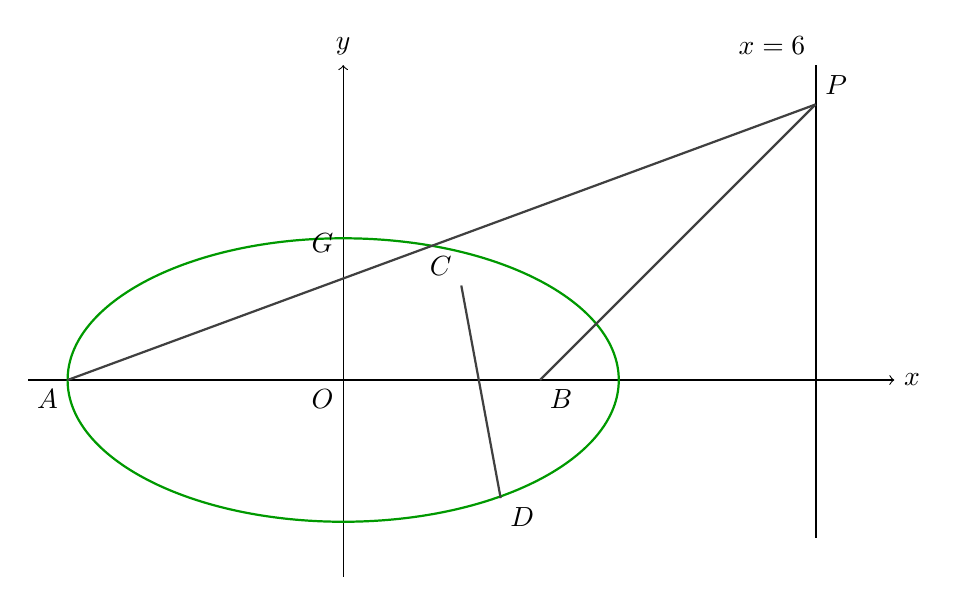
\begin{tikzpicture}[scale=1.0] % Adjust scale as needed for overall size

    % Define coordinates for key points (estimated from the image)
    \coordinate (O) at (0,0);
    \coordinate (A) at (-3.5,0);
    \coordinate (B) at (2.5,0);
    \coordinate (G) at (0,1.5); % Estimate for G, slightly above y-axis intersection
    \coordinate (C) at (1.5,1.2); % Point on ellipse
    \coordinate (D) at (2,-1.5); % Point on ellipse
    \coordinate (P) at (6,3.5); % Point on x=6 line

    % Draw the axes
    \draw[->] (-4,0) -- (7,0) node[right] {$x$};
    \draw[->] (0,-2.5) -- (0,4) node[above] {$y$};

    % Draw the ellipse (center, x-radius, y-radius) - estimated
    \draw[green!60!black, thick] (0,0) ellipse (3.5cm and 1.8cm);

    % Draw the vertical line x=6
    \draw[thick] (6,-2) -- (6,4) node[above left] {$x=6$};

    % Draw the lines connecting points
    \draw[thick, gray!50!black] (A) -- (P); % AP
    \draw[thick, gray!50!black] (B) -- (P); % BP
    \draw[thick, gray!50!black] (C) -- (D); % CD

    % Label the points
    \node at (O) [below left] {$O$};
    \node at (A) [below left] {$A$};
    \node at (B) [below right] {$B$};
    \node at (C) [above left] {$C$};
    \node at (D) [below right] {$D$};
    \node at (G) [above left] {$G$};
    \node at (P) [above right] {$P$};

\end{tikzpicture}
\end{center}



\chapter{Phrase}
\section{Type de phrase}
\begin{table}[H]
\centering
\begin{tabular}{|l|l|l|}
\hline
\rowcolor{cyan!20}
\textbf{TYPE DE PHRASE} & \textbf{SOUS-TYPE} & \textbf{EXEMPLES} \\
\hline
déclarative & — & \textit{Marie a lu ces livres.} \\
& & \textit{Marie a lu ces livres ?} \\
& & \textit{Marie a lu ces livres !} \\
\hline
désidérative & impératif & \textit{Lis davantage de livres !} \\
\cline{2-3}
& subjonctif & \textit{Que Marie lise ces livres !} \\
& & \textit{Puisse Marie réussir !} \\
\hline
exclamative & à mot exclamatif & \textit{Comme Marie semble heureuse !} \\
& & \textit{Quelle chance elle a !} \\
\cline{2-3}
& à mot intensif-exclamatif & \textit{Marie a lu tant de livres !} \\
& & \textit{Paul a un tel courage !} \\
\hline
interrogative & partielle & \textit{Quels livres Marie a lus ?} \\
& & \textit{Qui est venu ?} \\
\cline{2-3}
& totale & \textit{Est-ce que Marie a lu ces livres ?} \\
& & \textit{Marie a-t-elle lu ces livres ?} \\
& & \textit{A-t-elle lu ces livres ?} \\
\hline
\end{tabular}
\end{table}

\begin{enumerate}
    \item désidératives
    \begin{enumerate}
        \item 第一三人称不用impératif,用subjonctif introduit par \textit{que}
        \begin{itemize}
            \item Qu’il vienne !
            \item Que je sois pendu si je comprends ce qui se passe !
        \end{itemize}
        \item subjonctif不加que也属于正式用法
        \begin{enumerate}
            \item souhait
            \begin{itemize}
                \item Puisse-t-elle lui donner la même éducation que Gunilla à Victor
            \end{itemize}
            \item regret
            \begin{itemize}
                \item Plût au ciel qu’il soit venu !
            \end{itemize}
        \end{enumerate}
        \item impératif用法强调une réalisation ou une action future
        \begin{enumerate}
            \item injonction
            \begin{itemize}
                \item Sortons !
            \end{itemize}
            \item souhait
            \begin{itemize}
                \item Dormez bien !
            \end{itemize}
        \end{enumerate}
        \item subjonctif用法强调愿望表达不一定以现实可行性为前提
        \begin{enumerate}
            \item injonction
            \begin{itemize}
                \item Qu’il vienne !
            \end{itemize}
            \item souhait
            \begin{itemize}
                \item Que la force soit avec toi !
            \end{itemize}
            \item imprécation
            \begin{itemize}
                \item Que je sois pendu si je comprends ce qui se passe !
            \end{itemize}
        \end{enumerate}
    \end{enumerate}
\end{enumerate}

\subsection{Les formes des types de phrases indépendantes}
\begin{table}[H]
\centering
\begin{tabular}{|l|p{0.35\textwidth}|p{0.45\textwidth}|}
\hline
\rowcolor{cyan!20}
\textbf{TYPE DE PHRASE} & \textbf{FORME DU VERBE} & \textbf{AUTRE ÉLÉMENT LEXICAL} \\
\hline
déclarative & $-$ indicatif (\textit{Paul viendra.}) & $-$ \\
& $-$ infinitif (\textit{Et Paul de sursauter.}) & \\
\hline
désidérative & $-$ impératif (\textit{Venez ici !}) & $-$ \textit{que} + subjonctif (\textit{Qu'il vienne !}) \\
& $-$ subjonctif à sujet inversé ou suffixé (\textit{Puisse Marie vous entendre !}) & $-$ \textit{pourvu que} + subjonctif (\textit{Pourvu qu'il vienne !}) \\
\hline
exclamative & $-$ indicatif (\textit{Comme il pleut !}) & $-$ mot exclamatif : \textit{ce que, combien, comme, comment, que, quel, qu'est-ce que} \\
& $-$ infinitif (\textit{Paul, faire tant de bruit !})
& $-$ adverbe ou adjectif intensif-exclamatif : \textit{si, tant, tel, tellement} \\
\hline
interrogative & $-$ indicatif (\textit{Où allez-vous ?}) & $-$ mot interrogatif : \textit{combien, comment, lequel, où, pourquoi, quand, que, quel, qu'est-ce que, qu'est-ce qui, quoi, quoi, qui est-ce que, qui est-ce qui} \\
& $-$ indicatif à sujet suffixé (\textit{Viendrez-vous ?})
& $-$ introducteur : \textit{est-ce que} \\
\hline
\end{tabular}
\end{table}

\subsection{Les types de subordonnées complétives}


\begin{table}[H]
\centering
\begin{adjustbox}{max width=\textwidth}
    \begin{tabular}{|l|l|l|p{0.45\textwidth}|}
    \hline
    \rowcolor{cyan!20}
    \textbf{TYPE DE COMPLÉTIVE} & \textbf{INTRODUCTEUR} & \textbf{FORME DU VERBE} & \textbf{EXEMPLES} \\
    \hline
    déclarative & \textit{que} & indicatif ou subjonctif & \textit{Pierre pense [qu'elle a lu ces livres].} \\
    & & & \textit{Pierre regrette [qu'elle ait lu ces livres].} \\
    \hline
    désidérative & \textit{que} & subjonctif & \textit{Pierre ordonne [qu'elle lise ces livres].} \\
    & & & \textit{Pierre souhaite [qu'elle réussisse].} \\
    \hline
    interrogative & \textit{si} ou mot interrogatif & indicatif & \textit{Pierre se demande [quels livres elle a lus].} \\
    & & & \textit{Pierre se demande [qui est venu].} \\
    & & & \textit{Pierre se demande [si elle a lu ces livres].} \\
    \hline
    exclamative & \textit{que} ou mot exclamatif & indicatif ou subjonctif & \textit{Pierre sait [comme elle est heureuse].} \\
    & & & \textit{Pierre regrette [qu'elle soit si triste].} \\
    \hline
    \end{tabular}
\end{adjustbox}
\end{table} 









\subsection{Subordonnées déclaratives}
\subsubsection{La subordonnée déclarative sujet}
\begin{enumerate}
    \item 从句动词大多用subjonctif,个别用indicatif
    \begin{itemize}
        \item Que Paul soit absent m'étonne
        \item Ça m'étonne, que Paul soit absent
        \item Que la vie n'est pas rose en France et exige beaucoup d'opiniâtreté commence à se savoir
    \end{itemize}
    \item 可用Périphérique结构,主语用ce, cela, ça替代
    \begin{itemize}
        \item Ça m’étonne, que Paul soit absent
    \end{itemize}
    \item subordonnée sujet可倒置于动词后
    \begin{itemize}
        \item À cela s’ajoute qu’aucune décision n’a été prise
        \item D’où vient que Paul est en retard
        \item À quoi sert que vous ayez pris tant de précautions
    \end{itemize}
\end{enumerate}

\section{Les phrases verbales}
\subsection{La phrase à l’indicatif et au subjonctif}
\subsubsection{Le sujet}
\begin{enumerate}
    \item form de sujet
    \begin{enumerate}
        \item nom/pronom
        \item une phrase subordonnée
        \begin{itemize}
            \item Qu’il faille changer le papier peint ennuie le locataire
        \end{itemize}
        \item un syntagme à l’infinitif
        \begin{itemize}
            \item Réserver votre billet par Internet est impossible actuellement.
        \end{itemize}
    \end{enumerate}
    \item sujet inversé
    \begin{enumerate}
        \item 主语过长
        \begin{itemize}
            \item Ont été désignés pour cette mission Luc, Jean et Paul
        \end{itemize}
        \item interrogatives
        \begin{itemize}
            \item Où va Paul
        \end{itemize}
        \item exclamatives
        \begin{itemize}
            \item Quelle chance a Paul
        \end{itemize}
        \item certaines phrases au subjonctif
        \begin{itemize}
            \item Puisse Paul nous aider
        \end{itemize}
    \end{enumerate}
    \item sujet omis:大部分是verbes impersonnels;\textit{mieux vaut, peu importe, voici}
    \begin{itemize}
        \item Peu importe les conséquences.
        \item Faudrait prendre un peu plus de temps.
        \item Suffit qu’elle veuille, dit Joseph
    \end{itemize}
    \begin{enumerate}
        \item sujet omis的情况下,ne也应该省略,除了n’empêche和n’importe这个固定搭配
        \begin{itemize}
            \item N’empêche que tu aurais pu faire attention.
            \item Faut pas exagérer !
        \end{itemize}
    \end{enumerate}
\end{enumerate}

\subsubsection{Les compléments}

\begin{table}[H]
    \centering
    
    \begin{adjustbox}{max width=\textwidth}
        \begin{tabular}{|l|p{0.2\textwidth}|>{\RaggedRight}p{0.25\textwidth}|>{\RaggedRight}p{0.25\textwidth}|}
        \hline
        \rowcolor{cyan!20}
        \textbf{CATÉGORIE} & \textbf{ATTRIBUT} & \RaggedRight \textbf{COMPLÉMENT DIRECT} & \textbf{COMPLÉMENT OBLIQUE} \\
        \hline
        adjectif ou syntagme adjectival & \textit{Paul est [content].} & \textit{Ce tableau coute [cher].} & \textit{Luc vend [cher] ce tableau.} \\
        \hline
        adverbe ou syntagme adverbial & \textit{Ce tableau est [mieux].} & \textit{Celui-ci coute [davantage].} & \textit{Luc va [très bien].} \\
        \hline
        syntagme nominal & \textit{Paul est [mon ami].} & \textit{Paul mange [la pomme].} & \textit{Luc va [rue Madame].} \\
        \hline
        syntagme prépositionnel & \textit{Paul est [en forme].} & $-$ & \textit{Luc pense [à Marie].} \\
        \hline
        syntagme verbal & \textit{Ce tableau est [à vendre].} & \textit{Paul veut [venir demain].} & \textit{Luc va [faire les courses].} \\
        \hline
        phrase subordonnée & $-$ & \textit{Paul veut [que tu viennes].} & \textit{Je me souviens [qu'il neigeait].} \\
        \hline
        \end{tabular}
    \end{adjustbox}
\end{table}



\subsubsection{Les ajouts}
\begin{enumerate}
    \item adverbe ou syntagme adverbial
    \begin{itemize}
        \item Paul travaille [bien]
    \end{itemize}
    \item syntagme prépositionnel
    \begin{itemize}
        \item Paul garde espoir [malgré la crise]
    \end{itemize}
    \item adjectif ou syntagme adjectival invariable ou lié à un nom
    \begin{itemize}
        \item Lou a refusé [net]
        \item Lou est partie [furieuse]
    \end{itemize}
    \item syntagme nominal
    \begin{itemize}
        \item Paul travaille [le samedi]
    \end{itemize}
    \item pronom contrastif ou quantifieur
    \begin{itemize}
        \item Paul viendra, [lui]
        \item Les élèves viendront [tous]
    \end{itemize}
    \item syntagme verbal
    \begin{itemize}
        \item Haussant le ton, il est intervenu.
    \end{itemize}
    \item subordonnée circonstancielle, comparative, ou relative extraposée
    \begin{itemize}
        \item Alex viendra [quand il pourra]
        \item Alex ment [comme il respire].
        \item Des gens sont arrivés, [qui étaient énervés].
    \end{itemize}
    \item des incises ou commentaires 
    \begin{itemize}
        \item Lou a, [je crois], terminé son travail.
    \end{itemize}
    \item des termes d’adresse nominaux, des interjections ou des particules de discours
    \begin{itemize}
        \item Venez, [les enfants] !
        \item Tu peux me passer le sel, [s’il te plait] ?
    \end{itemize}
\end{enumerate}





\subsubsection{Les éléments en début de phrase verbale}
\begin{enumerate}
    \item élément marqueur:conjonction de coordination, subordonnant
    \item élément extrait:le mots, syntagmes interrogatifs ou exclamatifs
    \begin{enumerate}
        \item un pronom
        \begin{itemize}
            \item Qui Paul a-t-il rencontré hier ?
        \end{itemize}
        \item un syntagme nominal
        \begin{itemize}
            \item Quelle chance tu as !
        \end{itemize}
        \item un syntagme prépositionnel 
        \begin{itemize}
            \item À qui est-ce que vous pensez ?
        \end{itemize}
        \item un syntagme verbal
        \begin{itemize}
            \item Le laver, il faut.
        \end{itemize}
        \item un adjectif
        \begin{itemize}
            \item Quelle est la température ?
        \end{itemize}
        \item un adverbe
        \begin{itemize}
            \item Quand partiras-tu ?
        \end{itemize}
    \end{enumerate}
    \item un mot ou un syntagme ajout
    \item un mot ou un syntagme périphérique
    \begin{enumerate}
        \item nom, pronom ou syntagme nominal 
        \begin{itemize}
            \item Paul, on ne lui parle plus.
        \end{itemize}
        \item adjectif ou syntagme adjectival
        \begin{itemize}
            \item Plus grand que toi, personne ne peut l’être.
        \end{itemize}
        \item infinitif ou syntagme verbal
        \begin{itemize}
            \item Avoir vingt ans, ce n’est pas forcément le plus bel âge de la vie.
        \end{itemize}
        \item phrase subordonnée
        \begin{itemize}
            \item Que tu viennes demain, ça rassure tout le monde.
        \end{itemize}
    \end{enumerate}
\end{enumerate}

\begin{table}[H]
    \centering
    \begin{adjustbox}{max width =\textwidth}
        \begin{tabular}{|l|p{0.65\textwidth}|} % Adjust 0.65\textwidth as needed for your document layout
        \hline
        \rowcolor{cyan!20}
        \textbf{FONCTIONS} & \textbf{EXEMPLES} \\
        \hline
        MARQUEUR + EXTRAIT + AJOUT + PÉRIPHÉRIQUE & \textit{Mais comment, d'ailleurs, Paul, j'ai l'ai raté ?} \\
        MARQUEUR + EXTRAIT + PÉRIPHÉRIQUE + AJOUT & \textit{Mais comment, Paul, d'ailleurs, je l'ai raté ?} \\
        MARQUEUR + PÉRIPHÉRIQUE + EXTRAIT + AJOUT & \textit{Mais Paul, comment, d'ailleurs, je l'ai raté ?} \\
        MARQUEUR + PÉRIPHÉRIQUE + AJOUT + EXTRAIT & \textit{Mais Paul, d'ailleurs, comment je l'ai raté ?} \\
        MARQUEUR + AJOUT + PÉRIPHÉRIQUE + EXTRAIT & \textit{Mais d'ailleurs, Paul, comment je l'ai raté ?} \\
        MARQUEUR + AJOUT + EXTRAIT + PÉRIPHÉRIQUE & \textit{Mais d'ailleurs, comment, Paul, j'e l'ai raté ?} \\
        \hline
        EXTRAIT + PÉRIPHÉRIQUE + AJOUT + MARQUEUR & \textit{Comment Paul d'ailleurs est-ce que je l'ai raté?} \\
        EXTRAIT + AJOUT + MARQUEUR + PÉRIPHÉRIQUE & \textit{Comment d'ailleurs est-ce que Paul, je l'ai raté?} \\
        EXTRAIT + MARQUEUR + AJOUT + PÉRIPHÉRIQUE & \textit{Comment est-ce que d'ailleurs, Paul, je l'ai raté?} \\
        EXTRAIT + MARQUEUR + PÉRIPHÉRIQUE + AJOUT & \textit{Comment est-ce que Paul, d'ailleurs, je l'ai raté?} \\
        EXTRAIT + AJOUT + PÉRIPHÉRIQUE + MARQUEUR & \textit{Comment, d'ailleurs, Paul, est-ce que je l'ai raté?} \\
        EXTRAIT + PÉRIPHÉRIQUE + MARQUEUR + AJOUT & \textit{Comment, Paul, est-ce que d'ailleurs j'ai raté?} \\
        \hline
        PÉRIPHÉRIQUE + MARQUEUR + AJOUT + EXTRAIT & \textit{Moi, est-ce que, d'ailleurs, à Paul, j'ai parlé?} \\
        PÉRIPHÉRIQUE + AJOUT + EXTRAIT + MARQUEUR & \textit{Moi d'ailleurs, à Paul, est-ce que j'ai parlé?} \\
        PÉRIPHÉRIQUE + AJOUT + MARQUEUR + EXTRAIT & \textit{Moi d'ailleurs est-ce que à Paul, j'ai parlé?} \\
        PÉRIPHÉRIQUE + MARQUEUR + EXTRAIT + AJOUT & \textit{Moi, est-ce que, à Paul, d'ailleurs j'ai parlé?} \\
        PÉRIPHÉRIQUE + EXTRAIT + MARQUEUR + AJOUT & \textit{Moi, à Paul, est-ce que d'ailleurs j'ai parlé?} \\
        PÉRIPHÉRIQUE + EXTRAIT + AJOUT + MARQUEUR & \textit{Moi, à Paul, d'ailleurs, est-ce que j'ai parlé?} \\
        \hline
        \end{tabular}
    \end{adjustbox}
    \caption{\textbf{L'ordre des éléments en début de phrase}}
\end{table}

\subsection{La phrase à l’impératif}
\begin{enumerate}
    \item 无sujet syntaxique
    \item le, la, les, en, y替代complément时,它们要通过连字符置于动词后
    \begin{itemize}
        \item Apporte-le sur la table !
        \item Allons-y les amis !
    \end{itemize}
    \begin{enumerate}
        \item 否定句中proforme在动词前
        \begin{itemize}
            \item Ne l’apporte pas sur la table !
        \end{itemize}
    \end{enumerate}
    \item impératif只能是phrase indépendante,不能被subordonnant引导作为从句,但可被conjonction de coordination引导
\end{enumerate}

\subsection{Les phrases à l’infinitif et au participe présent}
\subsubsection{La phrase à l’infinitif}
不是句子而是syntagmes verbaux.
\begin{enumerate}
    \item sujet
    \begin{enumerate}
        \item syntagme nominal
        \begin{itemize}
            \item Et le silence de retomber 
        \end{itemize}
        \item nom propre
        \begin{itemize}
            \item Paul, se marier !
        \end{itemize}
        \item pronom fort
        \begin{itemize}
            \item Et lui de répliquer
        \end{itemize}
        \item 不能为弱形式
        \begin{itemize}
            \item *Et il de répliquer.
        \end{itemize}
    \end{enumerate}
    \item complement在动词后,但tout和rien在动词前
    \begin{itemize}
        \item Je lui ai dit d’arrêter [et lui de tout nier].
    \end{itemize}
    \item pas, 与其他副词一样置于动词前
    \begin{itemize}
        \item Paul, ne pas venir ?
        \item Et Paul de bien insister sur ce point.
    \end{itemize}
\end{enumerate}


\subsubsection{La phrase au participe présent}
\begin{enumerate}
    \item subordonnées circonstancielles de temps ou de cause
    \begin{itemize}
        \item L’hiver approchant, il faut rentrer les cactus.
        \item La discussion n’a pas pu aboutir, Paul ayant refusé de prendre part au vote
    \end{itemize}
    \item 被en引导时,不是subordonnées而是syntagme verbal
    \begin{itemize}
        \item En vieillissant, on comprend bien des choses.
    \end{itemize}
\end{enumerate}

\section{Les phrases subordonnées et coordonnées}
\subsection{Les subordonnées sujet ou complément}

\begin{table}[H]
    \centering
    \begin{tabular}{|p{2.5cm}|p{3.5cm}|>{\RaggedRight}p{2.5cm}|p{4.5cm}|}
    \hline
    \rowcolor{cyan!20}
    \textbf{TYPE} & \textbf{INTRODUCTEUR} & \textbf{MODE} & \textbf{FONCTION} \\
    \hline
    déclarative & \textit{que, de ce que} & indicatif ou subjonctif & sujet, complément direct ou oblique \\
    \hline
    désidérative & \textit{que, à de que} & subjonctif & sujet, complément direct ou oblique \\
    \hline
    interrogative & \textit{si}, mot, syntagme interrogatif & indicatif &  sujet, complément direct ou oblique \\
    \hline
    exclamative & mot, syntagme exclamatif, \textit{que} & indicatif ou subjonctif &  sujet, complément direct ou oblique \\
    \hline
    \end{tabular}
\end{table}

\subsubsection{Les subordonnées sujets}
\begin{enumerate}
    \item Le mode des déclaratives sujets大部分是subjonctif,但也可以是indicatif
    \begin{itemize}
        \item Qu’on n’arrête pas de grandir désespérait les mères, obligées de rallonger les robes d’une bande de tissu
        \item Qu’il faille chauffer en mai arrive rarement
    \end{itemize}
    \item la subordonnée sujet也可出现在动词后
    \begin{itemize}
        \item Plût au ciel qu’il pleuve
        \item À cela s’ajoute qu’aucune décision n’a été prise
        \item Si vous n’avez pas permis que je devienne bon, d’où vient que vous m’ayez ôté l’envie d’être méchant
    \end{itemize}
\end{enumerate}

\subsubsection{Les subordonnées compléments}
\begin{enumerate}
    \item 用le ou ça 指代complément direct
    \begin{itemize}
        \item Paul pense [que tout va bien].|Paul le pense
    \end{itemize}
    \item 用en ou y 指代complément oblique
    \begin{itemize}
        \item Il se souvient [que le président était encore vivant à ce moment-là].|Il s’en souvient
        \item On fait l’hypothèse [que l’atome est sécable].|On en fait l’hypothèse
        \item Paul est certain [qu’il a bien répondu].|Paul en est certain
        \item Elle songe [à ce que tout sera prêt].|Elle y songe
    \end{itemize}
    \item 可作为adverbes或prépositions的compléments,承担circonstancielle的功能
    \begin{itemize}
        \item Nous pouvons parler, encore que vous ayez l’air pressé
        \item Nous commencerons l’inventaire, avant que tu arrives
    \end{itemize}
\end{enumerate}

\subsection{Les subordonnées périphériques}
\begin{enumerate}
    \item 置于句首或句末,主句用ce, en, y等proforme指代
    \begin{itemize}
        \item Qu’il faille recourir au référendum, c’est probable
        \item Que vous soyez en avance, qui s’en plaindrait ?
        \item Si et quand on sortira de la crise, personne ne le sait
        \item Je trouve ça incroyable, comme il a changé
    \end{itemize}
    \item 在subordonnée interrogative ou exclamative中,更倾向于用 subordonnée périphérique而不是subordonnée sujet 
    \begin{itemize}
        \item C’est mieux [que tu partes].|?[Que tu partes] est mieux
        \item Ça m’est égal [avec qui il négocie].|?[Avec qui il négocie] m’est égal.
        \item Ça m’épate [comme il est malin].|*[Comme il est malin] m’épate.
    \end{itemize}
\end{enumerate}

\subsection{Les subordonnées ajouts}

\begin{table}[H]
    \centering

\begin{adjustbox}{max width =\textwidth}
    \begin{tabular}{|>{\RaggedRight}p{3cm}|>{\RaggedRight}p{5.5cm}|>{\RaggedRight}p{3.5cm}|>{\RaggedRight}p{5cm}|}
    \hline
    \rowcolor{cyan!20}
    \textbf{SUBORDONNÉE} & \textbf{INTRODUCTEUR} & \textbf{MODE} & \textbf{EXEMPLES} \\
    \hline
    circonstancielle & \textit{lorsque, que, si}, etc., mot ou syntagme antéposé, adverbe ou préposition + \textit{que} ou sans introducteur & indicatif, subjonctif, ou participe présent & Je viendrai [si je peux]. Il est fatigué [tant il travaille]. [Depuis qu'il est rentré], il ne peut rien faire. [Le temps pressant], on va rentrer. \\
    \hline
    comparative & \textit{que, comme} & indicatif & Il a plus travaillé [qu'on lui avait dit]. Il a travaillé [comme on lui avait dit]. \\
    \hline
    relative & \textit{dont, que, qui, où}, ou syntagme avec un mot relatif & indicatif ou subjonctif & la fille [que je vois] \newline un endroit [où j'irai] \newline une femme [à qui je puisse parler] \\
    \hline
    incise & sans introducteur & indicatif & Paul, [fit-il], est idiot. \\
    \hline
    \end{tabular}
\end{adjustbox}

\end{table}

\begin{enumerate}
    \item circonstancielles commencent
    \begin{enumerate}
        \item par adverbe
        \begin{itemize}
            \item l est fatigué, tant il travaille
        \end{itemize}
        \item par syntagme antéposé suivi de \textit{que}
        \begin{itemize}
            \item Aussi habile qu’il soit, il ne peut pas réussir.
        \end{itemize}
        \item sans introducteur, quand elles sont au participe présent ou au subjonctif avec un sujet suffixé
        \begin{itemize}
            \item Le temps pressant, on va rentrer.
            \item Je ne l’écouterai pas, fût-il ministre
        \end{itemize}
    \end{enumerate}
\end{enumerate}

\subsection{Les phrases coordonnées}

\subsection{Les phrases juxtaposées}

\subsubsection{Les phrases juxtaposées coordonnées}

\subsubsection{Les phrases juxtaposées subordonnées}
temporelle, causale, concessive, conditionnel
\begin{enumerate}
    \item participe présent
    \begin{itemize}
        \item Il faudra, [l’hiver approchant], rentrer les cactus
    \end{itemize}
    \item subjonctif avec sujet suffixé
    \begin{itemize}
        \item Le directeur, [eût-il été plus attentif ], ne pouvait tout contrôler.
    \end{itemize}
    \item imparfait
    \begin{itemize}
        \item N’était la difficulté à trouver à manger, les réfugiés se sentaient à l’abri.
    \end{itemize}
    \item conditionnel
    \begin{itemize}
        \item Me supplierait-il à genoux, je ne recevrai pas cet homme
    \end{itemize}
    \item Était-il heureux, il chantait.
    \item 第二个句子可以被que引导
    \begin{itemize}
        \item Était-il heureux, qu’il chantait
    \end{itemize}
\end{enumerate}


\section{Les phrases à extraction}
\subsection{Les différentes constructions à extraction}
\begin{enumerate}
    \item Les interrogatives partielles avec extraction:主句或从句
    \begin{itemize}
        \item À qui veux-tu parler ?
        \item Je me demande comment Paul va se rendre à Paris
    \end{itemize}
    \item Les exclamatives avec extraction:主句或从句
    \begin{itemize}
        \item On sait combien il s’est sacrifié pour ses enfants
        \item Que de mensonges il se croit obligé d’inventer
    \end{itemize}
    \item Les déclaratives avec extraction
    \begin{enumerate}
        \item Les antépositions avec inversion du sujet
        
        complément prépositionnel ou un adjectif attribut出现在句首,sujet在动词后 
        \begin{itemize}
            \item À cette potion amère, s’ajoute peu à peu un arrière-goût insidieux de mensonge.
            \item Rares sont ceux qui approuvent cette décision
            \item De ces contradictions si apparentes provient probablement le sentiment de malaise dont on ne peut se défaire tout au long de ce livre
        \end{itemize}
        \item Les antépositions sans inversion du sujet
        \begin{itemize}
            \item De cette affaire, on ne parle presque plus
            \item À cela, j’ai modestement pensé
            \item Légalement, ce dossier n’est pas défendable
        \end{itemize}
    \end{enumerate}
    \item Les subordonnées relatives et l’extraction
    \begin{itemize}
        \item Voici le livre auquel je pense
    \end{itemize}
    \begin{enumerate}
        \item Les relatives sans antécédent et l’extraction
        \begin{itemize}
            \item Tu peux inviter qui tu préfères
            \item Paul s’adressera à qui on lui conseillera de s’adresser
        \end{itemize}
    \end{enumerate}
    \item Les constructions clivées
    \item Les subordonnées circonstancielles avec extraction
    \begin{enumerate}
        \item Les circonstancielles de cause avec extraction
        
        tant, tellement引导的从句
        \begin{itemize}
            \item Nous connaissions les traits de son visage mieux que ceux de notre mère ou de notre femme, tant nous avions passé de temps à étudier ses photos, à les comparer
            \item Il ne pouvait pas bouger, tellement il était saisi
        \end{itemize}
        \item Les circonstancielles de concession avec extraction
        \begin{enumerate}
            \item 含pronom(quoi, qui que ce soit)的syntagme nominal ou prépositionnel后跟que
            \begin{itemize}
                \item Quoi que tu me dises, je ne changerai pas d’avis
                \item À qui que ce soit que je m’adresse, on me repousse
            \end{itemize}
            \item aussi/si/quelque/tout + syntagme adjectival ou adverbial + que;没有que时用sujet suffixé
            \begin{itemize}
                \item Joseph, disait-elle, tout intelligent qu’il était, avait aussi sa bêtise
                \item Si généreusement qu’il se comporte, il ne se rachètera pas auprès du public
                \item Il nous reste un espoir, si mince soit-il
            \end{itemize}
        \end{enumerate}
    \end{enumerate}
    \item Les comparatives avec extraction
    
    comme, que作为adverbes extraits
\end{enumerate}
\subsection{Les propriétés des phrases à extraction}

\subsubsection{La fonction de l’élément manquant}
\begin{enumerate}
    \item L’élément manquant correspond à un complément
    \begin{enumerate}
        \item complément de préposition作为extrait时不能没有préposition
        \begin{itemize}
            \item Pour quel projet as-tu voté ?
            \item * Quel projet as-tu voté pour ?
        \end{itemize}
    \end{enumerate}
    \item L’élément manquant correspond à un sujet
    
    当句首成分被看作是从句的主语时,它此时是extrait,从句被qui引导
    \begin{itemize}
        \item Quel genre de personne croyez-vous qui viendra ?
    \end{itemize}
    \item L’élément manquant correspond à un spécifieur
    \begin{itemize}
        \item Combien avez-vous d’enfants ? (combien d’enfants)
        \item Que vous avez de chance ! (que de chance,)
        \item Nous connaissions les traits de son visage mieux que ceux de notre mère ou de notre femme, tant nous avions passé de temps à étudier ses photos (tant de temp)
    \end{itemize}
    \item L’élément manquant correspond à un ajout
    \begin{itemize}
        \item Comment Paul travaille-t-il ?
        \item C’est l’endroit où Paul travaille.
        \item Pourquoi penses-tu qu’il vienne ?
    \end{itemize}
\end{enumerate}

\subsubsection{L’inversion du sujet dans les phrases à extraction}
\begin{itemize}
    \item Quel livre lit Paul en ce moment ?
    \item Je me demande quels livres lit Paul en ce moment
    \item J’ai lu le livre que lit Paul en ce moment
    \item  C’est ce livre que lisait Paul cet été
    \item Sur la place se dressait une cathédrale
    \item Il se conduit comme se conduisait son père
    \item Il faut y croire, si mince que paraisse cet espoir
\end{itemize}

\begin{enumerate}
    \item 疑问句中疑问词不再句首作为extrait时,不能用sujet inversé
    \begin{itemize}
        \item Paul viendra avec qui ?
        \item * Viendra Paul avec qui ?
    \end{itemize}
    \item extrait指代从句成分时,从句的主语可倒置
    \begin{itemize}
        \item Avec qui penses-tu que Paul viendra ?
        \item Avec qui penses-tu que viendra Paul ?
    \end{itemize}
\end{enumerate}


\subsubsection{La relation à distance entre l’élément extrait et l’élément manquant}
\begin{enumerate}
    \item 不能作为extraction的结构
    \begin{enumerate}
        \item les sujets infinitifs ou subordonnés
        \begin{itemize}
            \item Saluer ce voisin m’arrive rarement
            \item  * Quel voisin est-ce que [saluer ◊] t’arrive rarement ?
        \end{itemize}
        \item les compléments prépositionnels
        \item les subordonnées interrogatives
        \item les subordonnées relatives et les constructions clivées
        \item les subordonnées circonstancielles
    \end{enumerate}
    \item L’élément manquant appartient à un sujet
    \begin{enumerate}
        \item 名词是主语时,该名词的complément de nom可作为extrait
        \begin{itemize}
            \item  De quel livre [l’auteur ◊] est-il célèbre ?
        \end{itemize}
        \item 作为infinitif或subordonnée的动词是主语时,该动词的complément de verbe很难作为extrait
        \begin{itemize}
            \item Qu’on réduise l’espace réservé aux voitures est une de nos priorités
            \item * Quel espace [qu’on réduise ◊] est-il une de nos priorités ?
        \end{itemize}
    \end{enumerate}
    \item L’élément manquant appartient à un complément prépositionnel
    \begin{enumerate}
        \item préposition引导complément infinitif时可以extraire
        \begin{itemize}
            \item Je vais finir par résoudre ce problème
            \item Quel problème vas-tu finir [par résoudre ◊ SV] ?
        \end{itemize}
        \item préposition引导complément nominal很难extraire
        \begin{itemize}
            \item Je vais finir par un livre de cet auteur
            \item * De quel auteur vas-tu finir par un livre
        \end{itemize}
    \end{enumerate}
    \item L’élément manquant appartient à une subordonnée interrogative
    \begin{enumerate}
        \item complément d’une subordonnée interrogative à l’infinitif时可以extraction
        \begin{itemize}
            \item Quel problème savez-vous [comment expliquer ◊ ◊] ?
            \item Vous savez [comment expliquer ce problème ◊].
        \end{itemize}
        \item verb conjugué则难extraire
        \begin{itemize}
            \item * Quel problème savez-vous [comment le professeur a expliqué ◊ ◊] ?
        \end{itemize}
        \begin{enumerate}
            \item complément prépositionnel比complément nominal更容易extraire
            \begin{itemize}
                \item \% À quel problème savez-vous [si le professeur a pensé ◊] ?
            \end{itemize}
        \end{enumerate}
    \end{enumerate}
    \item L’élément manquant appartient à une circonstancielle
    \begin{enumerate}
        \item complement de verb conjugué很难extraire
        \begin{itemize}
            \item Tu seras soulagé [quand tu verras Pierre].
            \item * Qui seras-tu soulagé [quand tu verras ◊] ?
        \end{itemize}
        \item pour + infinitif结构的complement可以extraire
        \begin{itemize}
            \item Il a fallu trente ans [pour construire ce bâtiment].
            \item C’est un bâtiment qu’il a fallu trente ans [pour construire ◊].
        \end{itemize}
    \end{enumerate}
    \item L’élément manquant appartient à une subordonnée relative
    \begin{enumerate}
        \item L’extraction d’un second élément hors de la relative n’est pas possible
        \begin{itemize}
            \item Je connais un endroit [où acheter des cigarettes ◊].
            \item * Quel genre de cigarettes connais-tu un endroit [où acheter ◊ ◊] ?
            \item Je connais celui [qui a écrit ce livre].
            \item * Quel livre connais-tu celui [qui a écrit ◊] ?
        \end{itemize}
    \end{enumerate}
    \item L’élément extrait appartient à une coordination
    \begin{itemize}
        \item * Quels amis as-tu [appelés ◊ et invité leurs enfants] ?
        \item Quels amis as-tu [appelés ◊ et invités ◊] ?
    \end{itemize}
\end{enumerate}



\end{document}